\chapter{Hardware Layer: Memory Management for Next-Gen Interconnects}
\label{chap:hardware}
While \mind and \pulse implemented memory management functionality over Ethernet, and network-based resource disaggregation has gained traction due to advancements in network bandwidth, the inherent latency—limited by the speed of light—continues to impose significant overhead. Recent hardware advancements have led to the development of new-generation interconnects by major hardware vendors, such as Nvidia's NVLink~\cite{nvlink} and Intel's Compute Express Link (CXL)~\cite{cxl}. CXL, in particular, has emerged as a promising solution for expanding memory capacity and bandwidth by attaching external memory devices to PCIe slots, offering a dynamic and heterogeneous computing environment. Its low-latency and scalable nature make CXL an ideal interconnect for disaggregated architectures.

There are several fundamental differences between CXL and Ethernet, which we summarize below:
\begin{enumerate}[leftmargin=*, itemsep=0pt]
  \item \textbf{Data transfer mechanism}: Ethernet uses packet-based transmission, where data is encapsulated in frames with headers and footers, potentially increasing latency due to overhead. CXL, in contrast, provides memory semantics, enabling faster and more efficient data transfers without the overhead associated with packet framing.
  \item \textbf{Performance}: CXL offers orders of magnitude faster performance and provides significantly higher memory bandwidth compared to Ethernet.
  \item \textbf{Scale}: Current CXL prototypes~\cite{demystify,cxl2} are limited to operating within a single rack, whereas Ethernet can scale across entire data centers.
\end{enumerate}

Given these fundamental differences between the two interconnects, directly applying \mind's or \pulse's techniques to a CXL-based disaggregated architecture presents challenges. For instance, it is unclear whether an RMT-style packet switching network could be implemented within a CXL switch. This chapter explores the potential of next-generation interconnects like CXL and examines how the software stack must adapt to leverage these new technologies.

We begin by presenting an empirical study of the latest CXL ASIC prototypes and investigate their potential application in modern data center environments. We then discuss ongoing efforts to deploy CXL in real-world infrastructure and applications.


\begin{figure}[t]
    \centering
      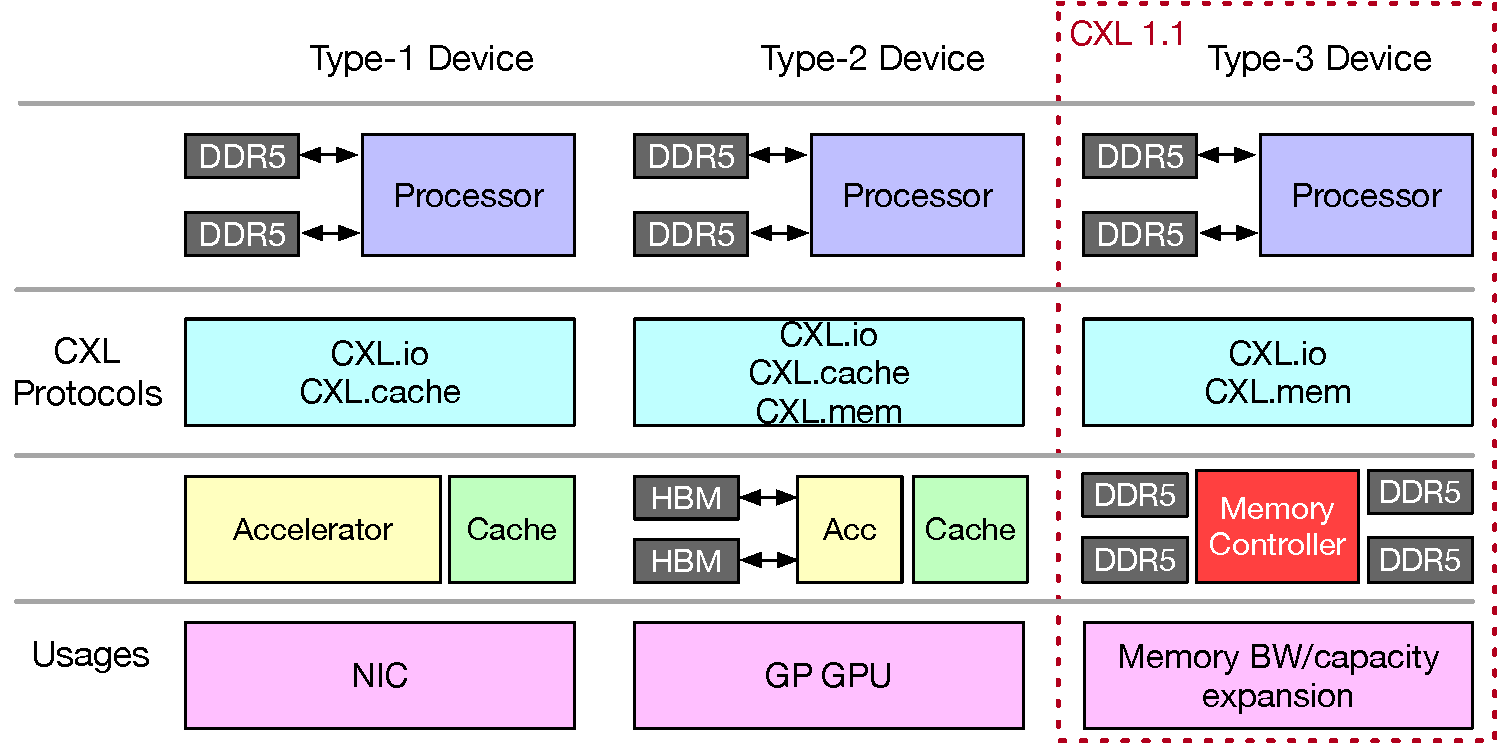
\includegraphics[width=0.8\columnwidth]{fig/cxl/cxl.pdf}
      \caption[CXL Overview]{\textbf{CXL Overview.} In this study, we focus on commercial CXL 1.1 Type-3 devices, leveraging CXL.io and CXL.mem protocols for memory expansion in single-server environments.} 
    \label{fig:cxl1.1} 
    \end{figure}


Our study aims to fill existing knowledge gaps by conducting detailed evaluations of CXL 1.1 for memory-intensive applications, leading to several \textit{intriguing observations}:
Contrary to the common perception that CXL memory, due to its higher latency, should be considered a separate, slower tier of memory~\cite{pond,tpp}, \textbf{we find that shifting some workloads to CXL memory can significantly enhance performance}, even if local memory's capacity and bandwidth are underutilized. This is because using CXL memory can decrease the overall memory access latency by alleviating bandwidth contention on DDR channels, thereby improving application performance.
From our analysis of application performance, we have formulated an abstract cost model (\S\ref{sec:cost}) that predicts substantial cost savings in practical deployments.

\section{Background and Methodology}
\label{sec:background}

This section presents an overview of CXL technology, followed by our experimental setup and methodologies.

\begin{figure*}[t]
    \centering
    \subfigure[CXL Server(socket 0 illustrated here).]{
      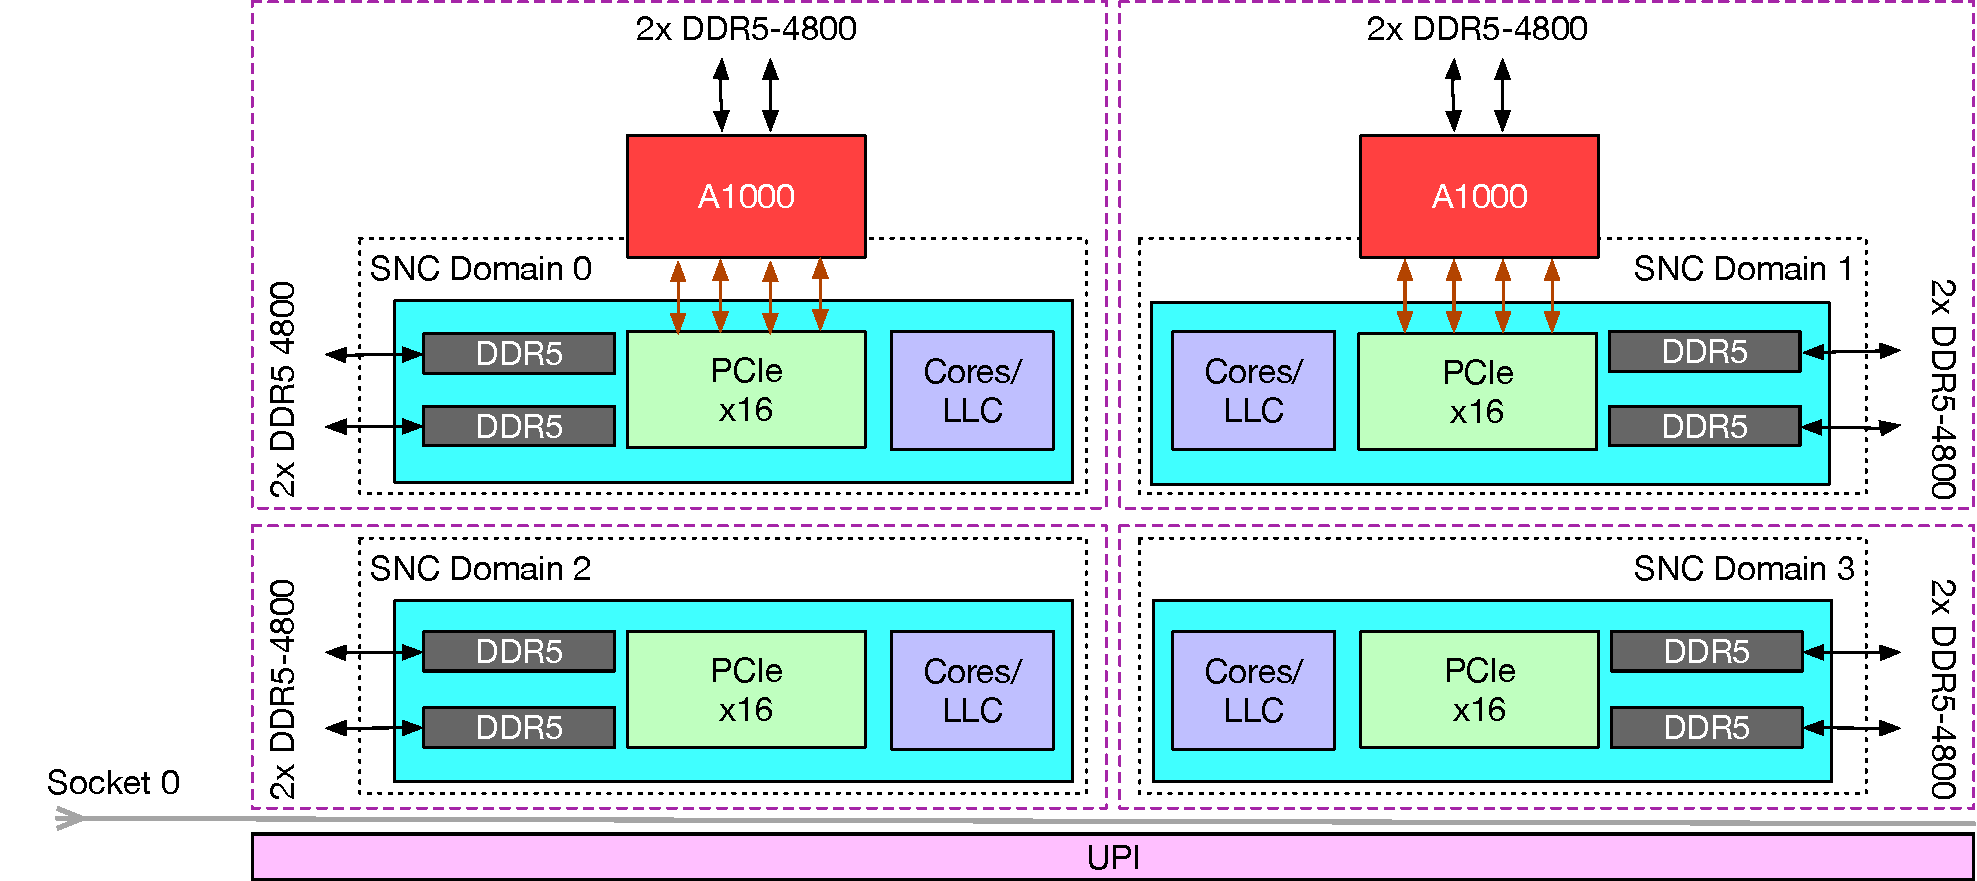
\includegraphics[width=0.65\textwidth]{fig/cxl/server.pdf}
      \label{fig:server}}
    \subfigure[Server setup.]{
      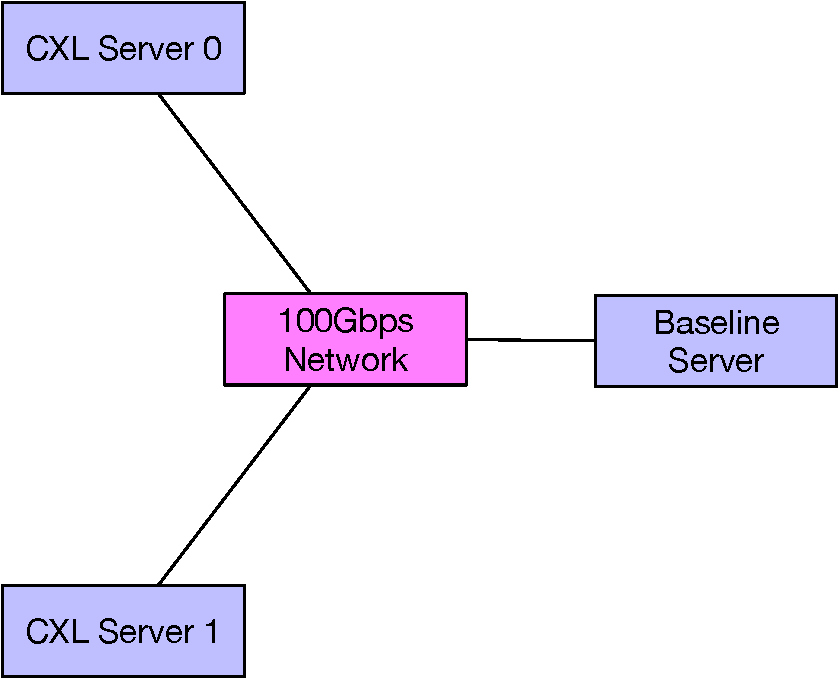
\includegraphics[width=0.31\textwidth]{fig/cxl/platform.pdf}
    \label{fig:platform}}
    \caption[CXL Experimental Platform]{\textbf{CXL Experimental Platform.} (a) Each CXL server is equipped with two A1000 memory expansion cards. SNC-4(\S\ref{ssec:config}) is enabled only for the raw performance benchmarks(\S\ref{sec:micro}) and bandwidth-bound benchmarks(\S\ref{sec:bandwidth}), and each SNC Domain is equipped with two DDR5 channels. (a) illustrates Socket 0; Socket 1 shares a similar setup except for the absence of CXL memory. (b) Our platform comprises two CXL servers and one baseline server. The baseline server replicates the same configuration but lacks any CXL memory cards.}
\end{figure*}

Compute Express Link (CXL) is a standardized interconnect technology that enables communication between processors and various devices, such as accelerators, memory expansion units, and smart I/O devices. CXL is built upon the physical layer of PCI Express® (PCIe®) 5.0~\cite{pcie5.0}, offering native support for x16, x8, and x4 link widths with data rates of $32.0$ GT/s and $64.0$ GT/s. The CXL transaction layer is implemented through three protocols: CXL.io, CXL.cache, and CXL.mem, as shown in Fig.~\ref{fig:cxl1.1}. The \textit{CXL.io} protocol, based on PCIe 5.0, handles device discovery, configuration, initialization, I/O virtualization, and direct memory access (DMA). \textit{CXL.cache} enables CXL devices to access the host processor's memory, while \textit{CXL.mem} allows the host to access device-attached memory using load/store commands.

CXL devices are classified into three types, each suited to specific use cases:
\begin{enumerate}[leftmargin=*, itemsep=0pt]
    \item \textit{Type-1 devices}, such as SmartNICs, utilize CXL.io and CXL.cache for communication with DDR memory.
    \item \textit{Type-2 devices}, including GPUs, ASICs, and FPGAs, use CXL.io, CXL.cache, and CXL.mem to share memory with the processor, enhancing workloads within the same cache domain.
    \item \textit{Type-3 devices} leverage CXL.io and CXL.mem for memory expansion and pooling, allowing for increased DRAM capacity, enhanced memory bandwidth, and the addition of persistent memory without occupying DRAM slots. These devices augment DRAM with CXL-enabled solutions, providing high-speed, low-latency storage.
\end{enumerate}

The current commercially available version of CXL is 1.1, which limits each CXL 1.1 device to function as a single logical device accessible by only one host at a time. Future generations, such as CXL 2.0, are expected to support partitioning devices into multiple logical units, allowing up to 16 different hosts to access separate portions of memory~\cite{sharma2023introduction}. In this work, we focus on commercially available CXL 1.1 Type-3 devices, specifically addressing their use for single-host memory expansion.



\subsection{Hardware Support for CXL}
\label{ssec:cxlhardware}

Recent announcements have introduced CXL 1.1 support for Intel Sapphire Rapids processors (SPR)~\cite{SPR} and AMD Zen 4 EPYC "Genoa" and "Bergamo" processors~\cite{amdgenoabergamo}. While commercial CXL memory modules are available from vendors such as Asteralabs~\cite{A1000}, Montage~\cite{mxc}, Micron~\cite{micron}, and Samsung~\cite{smt}, CXL memory expanders are still primarily in the prototype stage, with limited samples available, making access difficult for university research labs. As a result, due to the scarcity of CXL hardware, much of the research into CXL memory has relied on NUMA-based emulation~\cite{pond,tpp} and FPGA implementations~\cite{demystify, directcxl}, each presenting certain limitations:

\paragraphb{NUMA-based emulation} Given the cache-coherent nature and comparable transfer speeds between CXL and UPI/xGMI interconnects, NUMA-based emulation~\cite{pond, tpp} has been widely adopted for rapid application performance analysis and software prototyping. In this approach, CXL memory is exposed as a remote NUMA node. However, NUMA-based emulation fails to capture the precise performance characteristics of CXL memory due to inherent differences between CXL and UPI/xGMI interconnects~\cite{cxldatabase}, as highlighted in previous research~\cite{demystify}.

\paragraphb{FPGA-based implementation} Some hardware vendors, including Intel, use FPGA hardware to implement CXL protocols~\cite{intelfpga}, overcoming the performance inconsistencies of NUMA-based emulation. However, FPGA-based CXL memory implementations do not fully exploit memory chip performance due to the lower operating frequencies of FPGAs compared to ASICs~\cite{fpgaasic}. While FPGAs offer flexibility, they prioritize versatility over performance, making them suitable for early-stage CXL memory validation but not for production deployment. Intel’s recent evaluation~\cite{demystify} revealed several performance limitations in FPGA-based implementations, including reduced memory bandwidth during concurrent thread execution. This hampers rigorous evaluations for memory capacity- and bandwidth-bound applications, which are critical use cases for CXL memory expanders. A detailed discussion on the performance gap between CXL ASIC and FPGA controllers is provided in \S\ref{sec:micro}.

\subsection{Software Support for CXL}

\label{ssec:cxlsoftware}
While hardware vendors are actively advancing CXL production, a notable gap remains in software and OS kernel support for CXL memory. This deficiency has driven the development of specific software enhancements. We summarize the most recent patches in the Linux Kernel that add CXL-aware support, namely: (1) the interleaving policy support (unofficial) and (2) the hot page selection support (official since Linux Kernel v6.1).

\paragraphb{N:M Interleave Policy for Tiered Memory Nodes}

Traditional memory interleave policies distribute data evenly across memory banks, typically using a 1:1 ratio. However, with the emergence of tiered memory systems—where CPU-less memory nodes exhibit varying performance characteristics—new strategies are required to optimize memory bandwidth for bandwidth-intensive applications. The interleave patch~\cite{Interleavepatch} introduces an N:M interleave policy, which allows for the allocation of N pages to high-performance (top-tier) memory nodes and M pages to lower-tier nodes. For example, a 4:1 ratio directs $80\%$ of traffic to top-tier nodes and $20\%$ to lower-tier nodes. This ratio can be adjusted using the \texttt{vm.numa\_tier\_interleave} parameter. While the patch shows promising evaluation results~\cite{Interleavepatch}, the optimal memory distribution depends on specific hardware and application characteristics. Given the higher latency of CXL memory, as demonstrated in \S\ref{sec:micro}, performance-sensitive applications must be carefully profiled and benchmarked to fully leverage interleaving while mitigating potential performance trade-offs.

\paragraphb{NUMA Balancing \& Hot Page Selection}

The memory subsystem, now termed a memory tiering system, accommodates various memory types like PMEM and CXL memory, each with differing performance characteristics. To optimize system performance, frequently accessed "hot pages" should reside in faster memory tiers like DRAM, while less frequently accessed "cold pages" should be placed in slower tiers like CXL memory. Recent Linux Kernel patches address this:

\begin{enumerate}[leftmargin=*, itemsep=0pt]
    \item The \textit{NUMA-balancing} patch~\cite{numaautobalancing} implements a latency-aware page migration strategy that promotes recently accessed (MRU) pages by scanning NUMA balancing page tables and hinting at page faults. However, it may fail to accurately identify high-demand pages due to long scanning intervals, which could cause latency issues for certain workloads.
    \item The \textit{Hot Page Selection} patch~\cite{hot} introduces a Page Promotion Rate Limit (PPRL) mechanism to control the rate at which pages are promoted or demoted. While this extends the time for promotions/demotions, it improves workload latency by dynamically adjusting the hot page threshold to align with the promotion rate limit.
\end{enumerate}

Additionally, research prototypes like TPP~\cite{tpp} employ similar optimization concepts and are being considered for integration into the Linux Kernel~\cite{tpppatch}. However, during our testing with memory bandwidth-intensive applications, we encountered unexplained performance degradation with TPP. As a result, we rely on the well-tested kernel patches integrated into Linux Kernel since version 6.1.

\subsection{Experimental Platform Description}
Our evaluation testbed, illustrated in Fig. \ref{fig:platform}, consists of three servers. Two of these servers are dedicated to CXL experiments and are equipped with dual Intel Xeon 4th Generation CPUs (Sapphire Rapids, SPR), $1$ TB of 4800 MHz DDR5 memory, two $1.92$ TB SSDs, and two A1000 CXL Gen5 x16 ASIC memory expander modules from AsteraLabs, each equipped with $256$ GB of 4800 MHz memory (for a total of $512$ GB of memory per server). Both A1000 modules are attached to socket $0$. 

The third server serves as the baseline and is configured identically to the CXL experiment servers, except it lacks CXL memory expanders. It is used to initiate client requests and run workloads that strictly utilize main memory during application assessments. All servers are interconnected via $100$ Gbps Ethernet links.









\section{CXL 1.1 Performance Characteristics}
%\yupeng{Check the absolute value of each number}
\label{sec:micro}

In this section, we assess the performance of the CXL memory expander and compare it directly with main memory, which we designate as \textbf{MMEM} for clarity when contrasted against CXL memory. We analyze workload patterns and evaluate performance differences between local and remote socket scenarios.

\begin{figure}[t]
\centering
\subfigure[Local-socket MMEM]{
  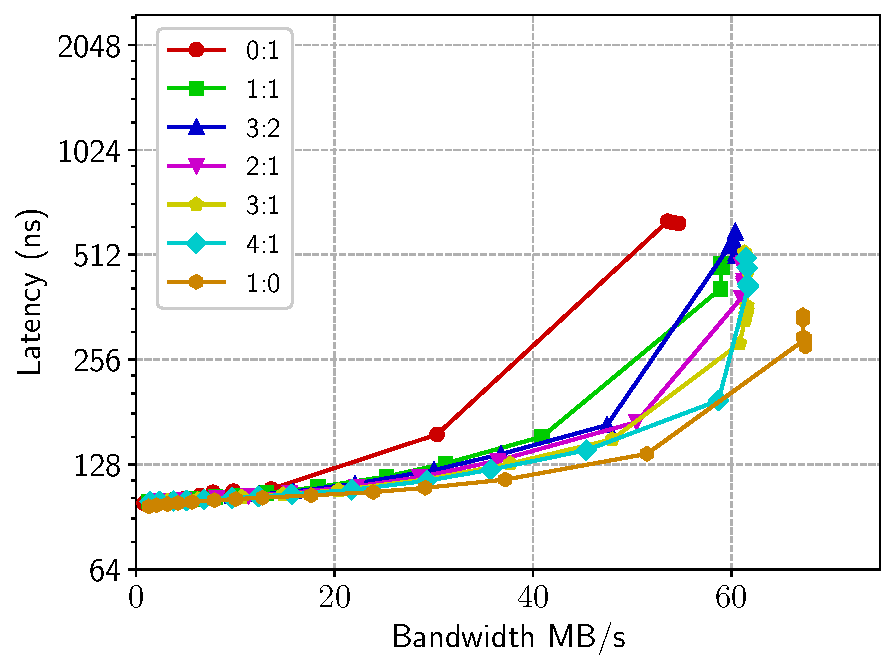
\includegraphics[width=0.25\textwidth]{fig/cxl/cxl_dram_workload_rw_c16_r0.pdf}
  \label{fig:localdram}}%
\subfigure[Remote-socket MMEM]{
  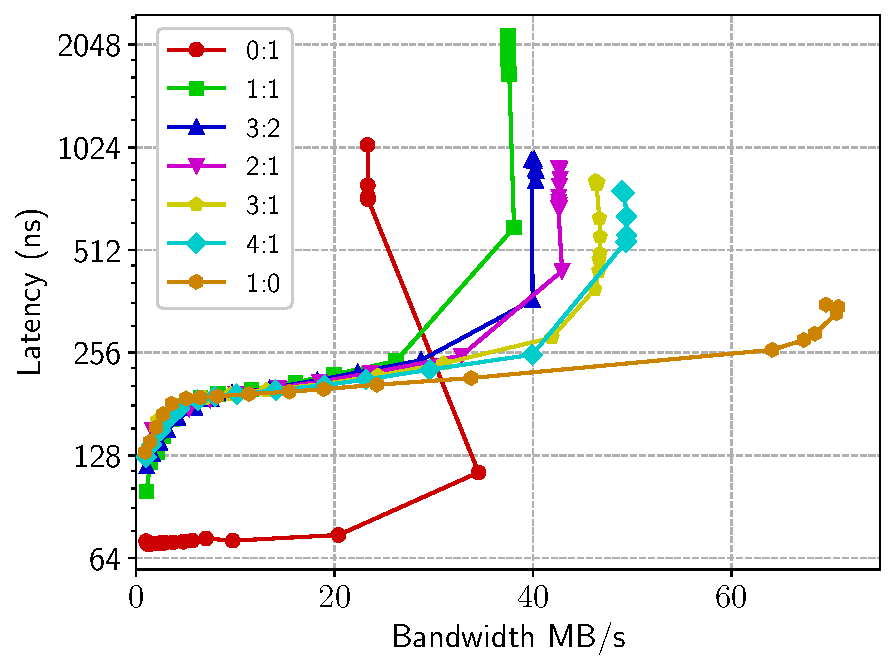
\includegraphics[width=0.25\textwidth]{fig/cxl/cxl_dram_workload_rw_c16_r0_rs.pdf}
  \label{fig:remotesocketdram}}% 
\subfigure[Local-socket CXL]{
  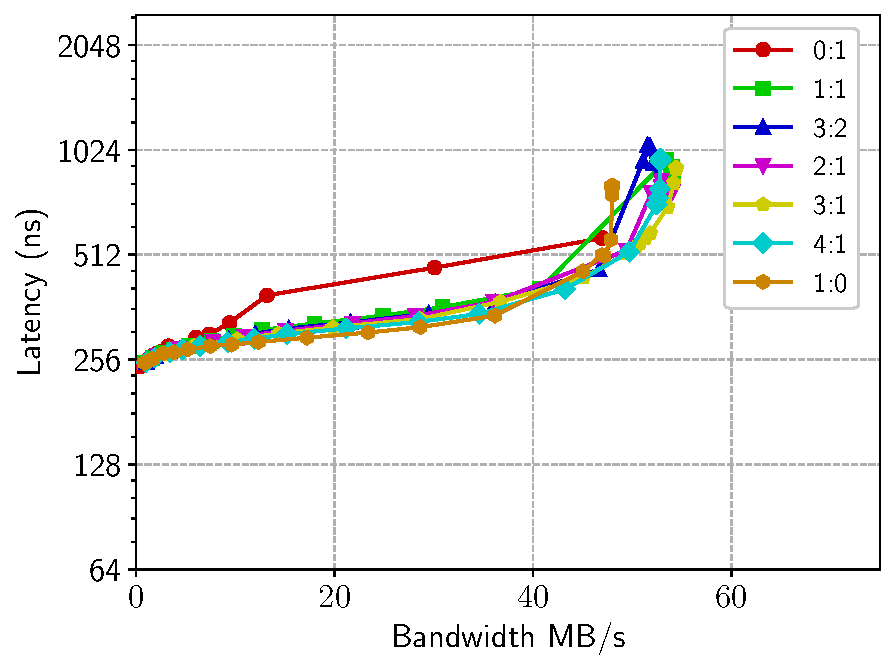
\includegraphics[width=0.25\textwidth]{fig/cxl/cxl_cxl_workload_rw_c16_r0.pdf}
  \label{fig:cxllocalsocket}}%
  \subfigure[Remote-socket CXL]{
  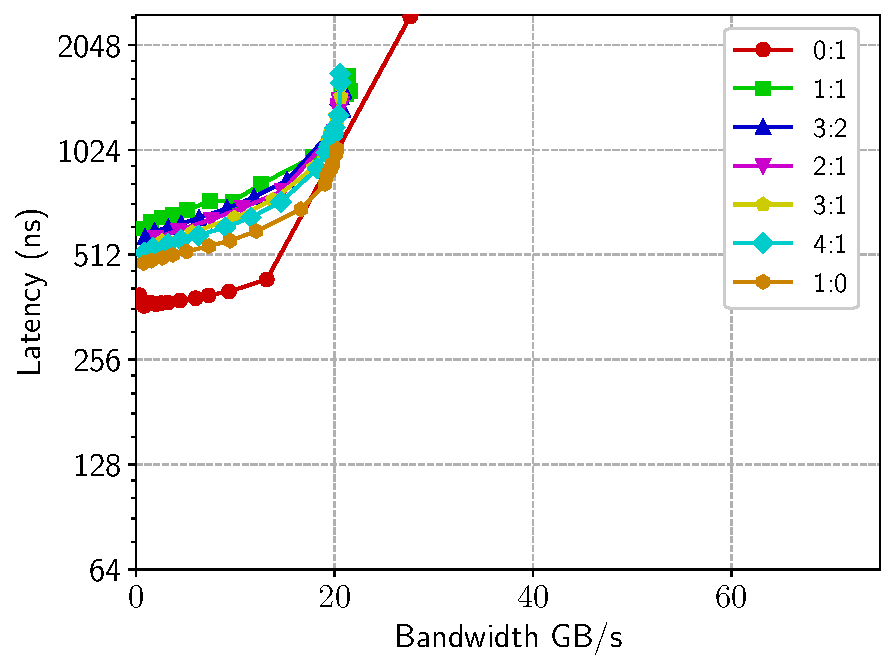
\includegraphics[width=0.25\textwidth]{fig/cxl/cxl_cxl_workload_rw_c16_r0_rs.pdf}
  \label{fig:cxlremotesocket}}%
 \caption[Overall effect of read-write ratio on MMEM and CXL across different distances]{\textbf{Overall effect of read-write ratio on MMEM and CXL across different distances.} The workloads are represented by read:write ratios (e.g., $0$:$1$ for write-only, $1$:$0$ for read-only). Accessing CXL memory locally incurs higher latency compared to MMEM but is more comparable to accessing MMEM on a remote socket. MMEM bandwidth peaks at $67$ GB/s, versus $54.6$ GB/s for CXL memory. Performance significantly declines when accessing CXL memory on a remote socket (\S\ref{ssec:performance}).  In specific scenarios, such as the write-only workload ($0$:$1$) in (b), the plot may show instances where bandwidth decreases and latency increases with heavier loads. The Y-axis is on a logarithmic scale.}
\label{fig:microbench-1}
\end{figure}

\begin{figure*}[t]
\centering
  \subfigure[Read-only workload]{
  % include first image
  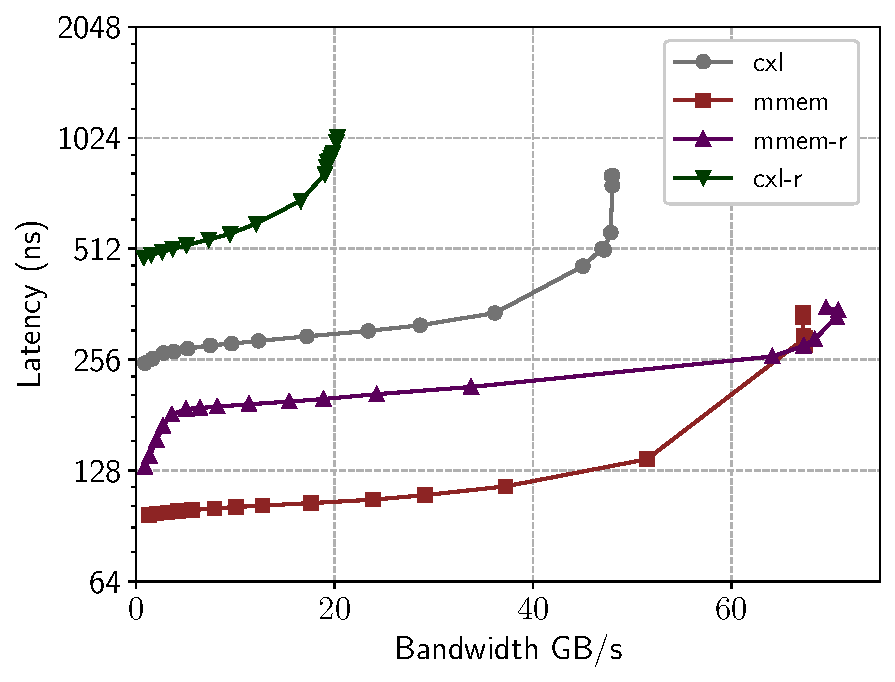
\includegraphics[width=0.25\textwidth]{fig/cxl/cxl_mix_workload0_c16_r0.pdf}
  \label{fig:readonly}}%
    \subfigure[Read:Write = $4$:$1$ workload]{
  % include first image
  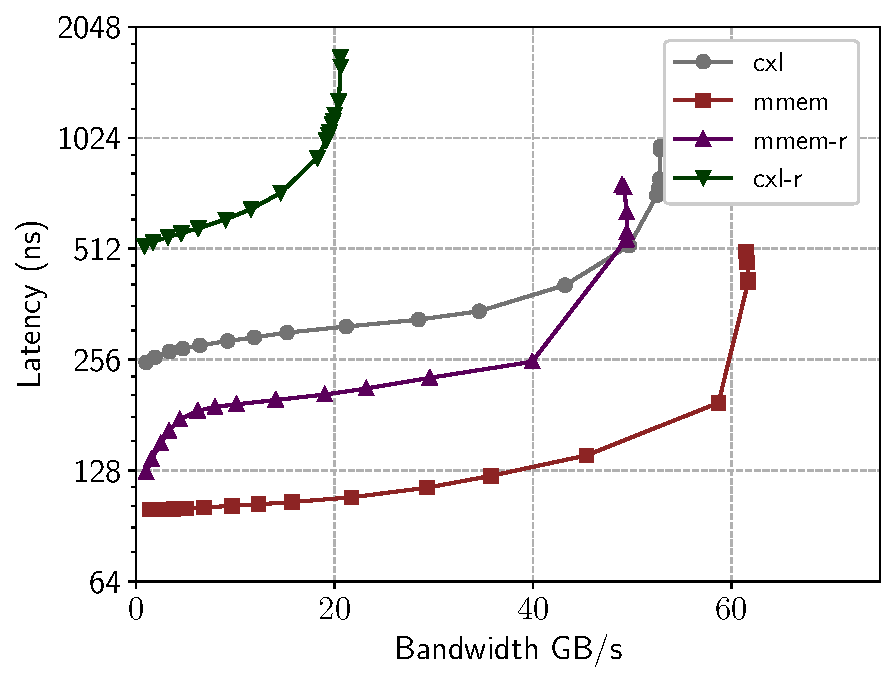
\includegraphics[width=0.25\textwidth]{fig/cxl/cxl_mix_workload12_c16_r0.pdf}
  \label{fig:readwrite41}}%
  \subfigure[Read:Write = $3$:$1$ workload]{
  % include first image
  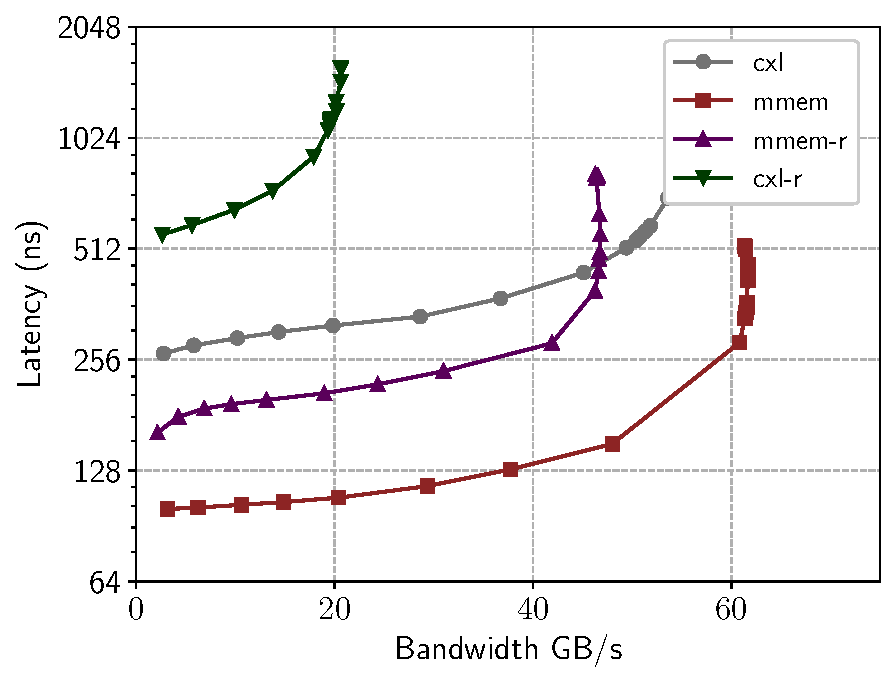
\includegraphics[width=0.25\textwidth]{fig/cxl/cxl_mix_workload3_c16_r0.pdf}
  \label{fig:readwrite31}}%
  \subfigure[Read:Write = $2$:$1$ workload]{
  % include first image
  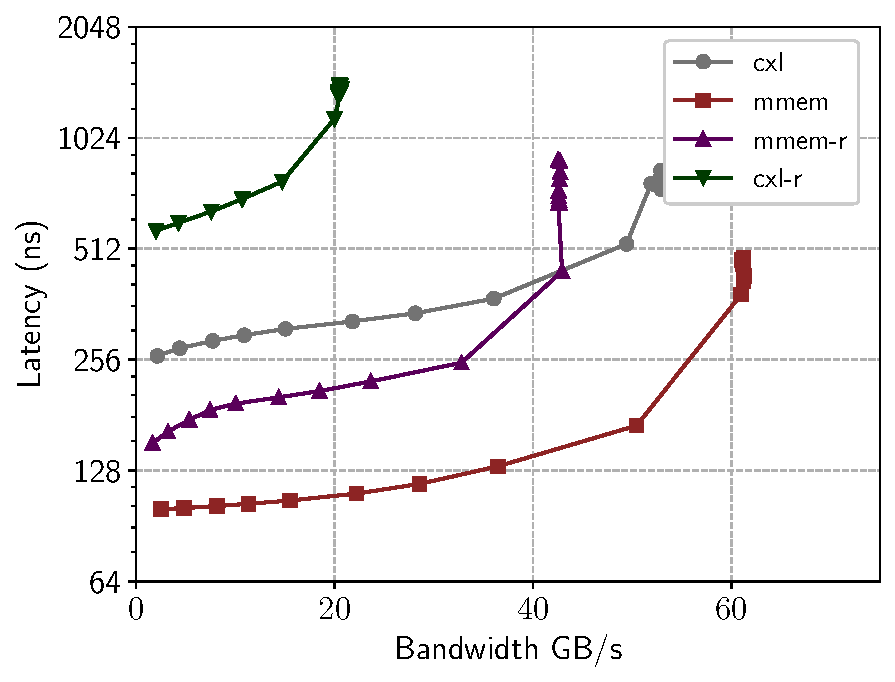
\includegraphics[width=0.25\textwidth]{fig/cxl/cxl_mix_workload2_c16_r0.pdf}
  \label{fig:readwrite21}}%
  \\
  \subfigure[Read:Write = $1$:$1$ workload]{
  % include first image
  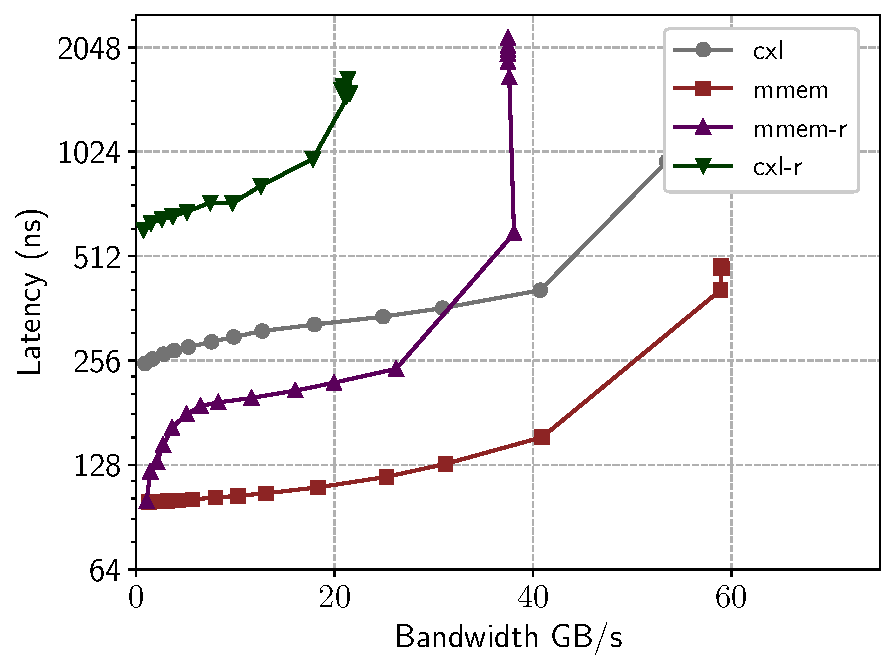
\includegraphics[width=0.25\textwidth]{fig/cxl/cxl_mix_workload5_c16_r0.pdf}
  \label{fig:readwrite11}}%
  \subfigure[Write-only workload]{
  % include first image
  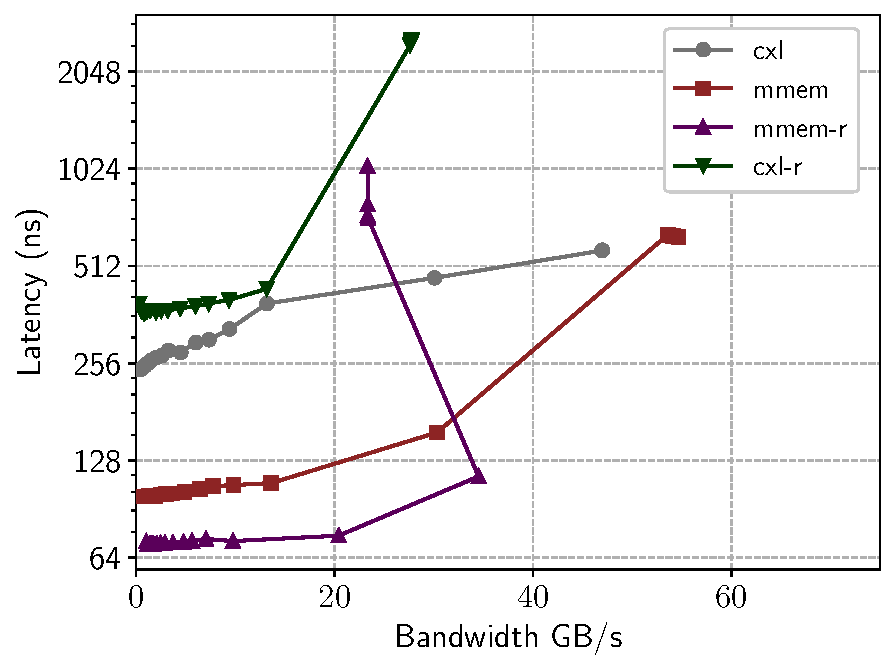
\includegraphics[width=0.25\textwidth]{fig/cxl/cxl_mix_workload6_c16_r0.pdf}
  \label{fig:writeonly}}%
  \subfigure[Read-only workload (random)]{
  % include first image
  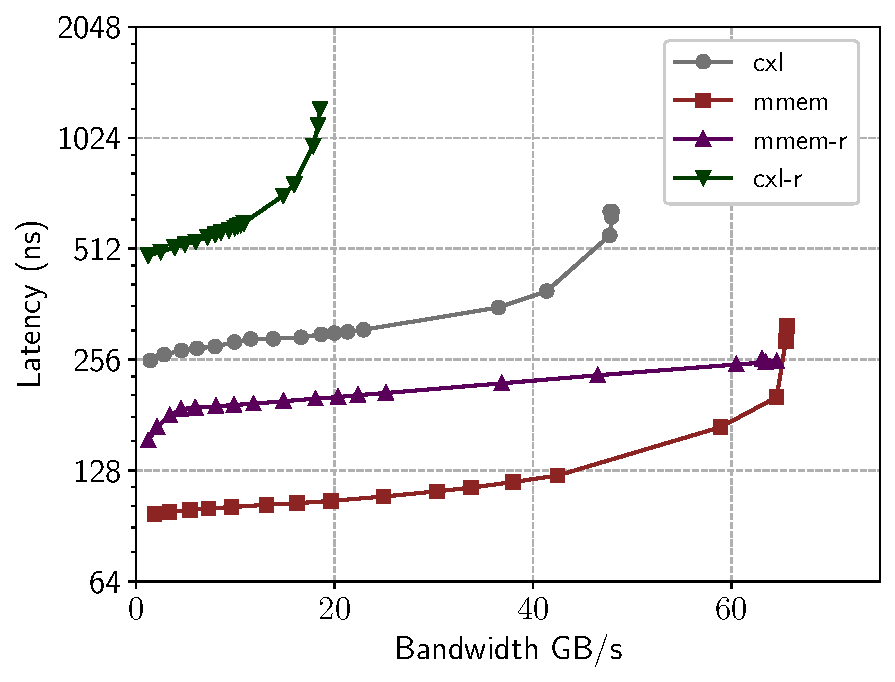
\includegraphics[width=0.25\textwidth]{fig/cxl/cxl_mix_workload0_c16_r1.pdf}
  \label{fig:readdatasize}}%
    \subfigure[Write-only workload (random)]{
  % include first image
  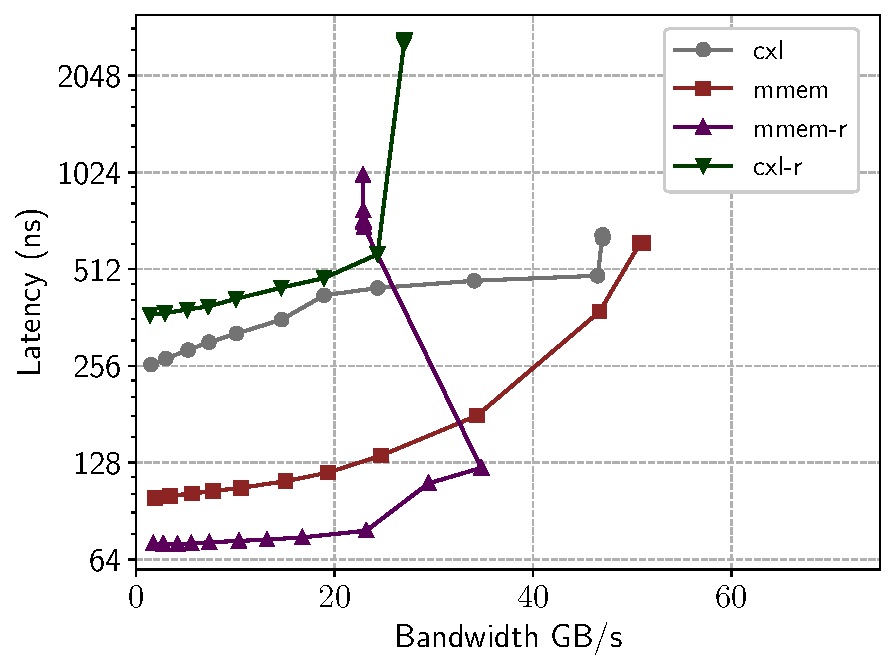
\includegraphics[width=0.25\textwidth]{fig/cxl/cxl_mix_workload6_c16_r1.pdf}
  \label{fig:writedatasize}}%
 \caption[A detailed comparison of MMEM versus CXL over diverse NUMA/socket distances and workloads]{\textbf{A detailed comparison of MMEM versus CXL over diverse NUMA/socket distances and workloads.} (a)-(f) shows the latency-bandwidth trend difference of accessing data from different distances in sequential access pattern, sorted by the proportion of write. We refer to main memory as \textbf{MMEM}, with MMEM-r and CXL-r representing remote socket MMEM and cxl memory access, respectively. The Y-axis is on a logarithmic scale.}
\label{fig:microbench-2}
\end{figure*}

\subsection{Experimental Configuration}
\label{ssec:config}
For each dual-channel A1000 ASIC CXL memory expander~\cite{A1000}, we connect two DDR5-4800 memory channels, providing a total capacity of $256$ GB. To ensure a fair comparison between MMEM and CXL-attached DDR5 memory, we use the Sub-NUMA Clustering (SNC)~\cite{snc} feature to equalize the number of memory channels in both configurations. 

\paragraphb{Sub-NUMA Clustering (SNC)} Sub-NUMA Clustering (SNC) is an enhancement over the traditional NUMA architecture, dividing a single NUMA node into smaller semi-independent sub-nodes (domains). Each sub-NUMA node has its own dedicated local memory, L3 caches, and CPU cores. In our experimental setup (Fig.~\ref{fig:server}), each CPU is partitioned into four sub-NUMA nodes. Each sub-NUMA node is equipped with two DDR5 memory channels connected to two $64$ GB DDR5-4800 DIMMs. SNC is enabled by setting the Integrated Memory Controllers (IMC) to 1-way interleaving. Based on specifications, a single DDR5-4800 channel has a theoretical peak bandwidth of $38.4$ GB/s~\cite{cxlcentric}, resulting in a combined memory bandwidth of up to $76.8$ GB/s per sub-NUMA node.

\paragraphb{Intel Memory Latency Checker (MLC)} We use Intel's Memory Latency Checker (MLC) to measure loaded-latency for various read-write workloads, employing a $64$-byte access size, consistent with prior work~\cite{demystify}. We deploy $16$ MLC threads, and while the thread count in MLC is configurable, it does not directly control memory request concurrency. Instead, MLC assigns distinct memory segments to each thread for simultaneous access. When evaluating loaded latency, MLC incrementally increases the operation rate per thread. Our results show that using $16$ threads with MLC accurately measures both idle and loaded latency, as well as the point at which bandwidth saturation occurs. MLC supports a wide range of workloads, including different read-write mixes and non-temporal writes.

Our study aims to address the following research questions:

\begin{itemize}
    \item How does the performance of CXL-attached memory compare to local-socket and remote-socket main memory?
    \item What is the performance impact of CXL memory under different read-write ratios and access patterns (random vs. sequential)?
    \item How do main memory and CXL memory behave under high memory load conditions?
\end{itemize}



\subsection{Basic Latency and Bandwidth Characteristics}
\label{ssec:performance}
This section presents our findings on memory access latency and bandwidth across different memory configurations: local-socket main memory (MMEM), remote-socket main memory (MMEM-r), CXL memory (CXL), and remote-socket CXL memory (CXL-r). Figure~\ref{fig:localdram} illustrates the loaded latency curve for MMEM under various read-write mixes. The read-only workload achieves a peak bandwidth of approximately $67$ GB/s, reaching $87\%$ of its theoretical maximum. However, as the proportion of write operations increases, bandwidth decreases, with write-only workloads dropping to $54.6$ GB/s. Initial memory latency is about $97$ ns, but it rises sharply as bandwidth nears full capacity, indicating bandwidth contention~\cite{cxl-centric, mt2}. Interestingly, latency starts increasing significantly at $75\%$-$83\%$ of bandwidth utilization, exceeding prior estimates of $60\%$ from earlier studies~\cite{cxl-centric}.

Figure~\ref{fig:remotesocketdram} compares latency for MMEM when accessed via a remote socket. For read-only workloads, latency starts around $130$ ns, whereas write-only workloads exhibit a much lower latency of $71.77$ ns. This reduction in latency for write-only operations stems from non-temporal writes, which proceed asynchronously without waiting for confirmation. While read-only tasks achieve similar maximum bandwidth to local MMEM, increasing the proportion of write operations drastically reduces bandwidth due to additional UPI traffic generated by cache coherence protocols. Notably, write-only workloads generate minimal UPI traffic but suffer from the lowest bandwidth because they utilize only one direction of the UPI’s bidirectional capacity. Moreover, latency escalation occurs earlier in remote-socket memory accesses than in local-socket ones, primarily due to queue contention at the memory controller.

Figure~\ref{fig:cxllocalsocket} illustrates the latency curve for CXL memory expansion, showing a minimum latency of $250.42$ ns. Despite the added overhead from PCIe and the CXL memory controller, CXL follows a similar "bandwidth contention" pattern as MMEM. Latency remains relatively stable as bandwidth increases, with a maximum of $56.7$ GB/s achieved under a $2:1$ read-write ratio. The lower maximum bandwidth compared to DRAM is attributed to PCIe overhead, such as additional headers. For read-only workloads, the maximum bandwidth is further reduced due to PCIe’s bidirectional nature, preventing full bandwidth utilization. Figure~\ref{fig:cxlremotesocket} displays the latency-bandwidth relationship for remote-socket CXL access, revealing an idle latency as high as $485$ ns. Additionally, maximum memory bandwidth is unexpectedly halved, reaching only $20.4$ GB/s under a $2:1$ read-write ratio— a much more severe performance drop compared to remote-socket MMEM (Fig.~\ref{fig:cxlremotesocket}). Since read-only access to a CXL Type-3 device on a remote socket does not generate significant coherence traffic, cache coherence can be ruled out as a cause. Further investigation using Intel Performance Counter Monitor (PCM)~\cite{pcm} confirmed that UPI utilization remained consistently below $30\%$. Discussions with Intel suggest this bottleneck likely stems from limitations in the Remote Snoop Filter (RSF) on the current CPU platform, which may be addressed in next-generation processors~\cite{emerald_rapids}.

\subsection{Different Read-Write Ratios \& Access Patterns}

Figures~\ref{fig:readonly}--\ref{fig:writeonly} compare performance under various read-write ratios. The results support our earlier observation that accessing CXL from a remote socket results in significantly higher latency and lower bandwidth. When accessing CXL from the same socket, latency is $2.4$-$2.6$ times that of local DDR and $1.5$-$1.92$ times that of remote-socket DDR. This suggests that directly running applications on CXL memory could severely degrade performance. However, for workloads spanning multiple NUMA nodes within the same socket, accessing CXL locally is comparable to accessing remote NUMA node memory. Additionally, as the proportion of write operations in the workload increases, the latency-bandwidth knee-point shifts left. Figures~\ref{fig:readdatasize} and~\ref{fig:writedatasize} show performance for read-only and write-only workloads under random access patterns. No significant performance differences were observed in these conditions.

\subsection{Key Insights}
\paragraphb{Avoiding Remote Socket CXL Access.}
CXL memory expansion is commonly used for memory-intensive applications, particularly those limited by memory capacity or bandwidth. In such cases, cross-socket memory access is not uncommon. However, developers should be aware of the performance drop when accessing CXL memory from a remote socket and avoid cross-socket CXL accesses where possible. Hardware vendors must also ensure compatibility between CXL memory modules and processors’ CXL support through cooperative testing. With full CXL 1.1 support, we expect the bandwidth attainable when accessing CXL across sockets to approach that of MMEM across sockets.

\paragraphb{Bandwidth Contention.}
Previous research~\cite{mt2, cxlcentric} highlighted the impact of bandwidth contention. We further examined how memory latency changes with varying read-write ratios under bandwidth contention. Latency remains stable at low to moderate bandwidth utilization but increases sharply as utilization approaches higher levels, primarily due to queuing delays in the memory controller~\cite{cxl-centric}. Additionally, when workloads include a higher proportion of write operations, the knee-point in latency occurs at lower memory bandwidth. While CXL memory is often described as a "tiered memory" solution, suitable only when MMEM is fully utilized~\cite{demystify, tpppatch, Interleavepatch}, we argue against this view. Even if MMEM bandwidth is underutilized (e.g., by $30\%$), offloading part of the workload (e.g., $20\%$) to CXL memory can yield overall performance improvements. We recommend treating CXL memory as a valuable resource for load balancing, even when local DRAM bandwidth is not fully utilized. Further real-world evaluations support this insight (\S\ref{sec:bandwidth}).

\paragraphb{Comparison with FPGA-based CXL Implementations.}
Intel recently disclosed performance metrics for their FPGA-based CXL prototype~\cite{demystify}. While they highlighted relative latency and bandwidth for soft and hard IP implementations, they did not share performance under load. Our measurements show that the ASIC CXL solution introduces only a $2.5\times$ latency overhead compared to MMEM, surpassing most of Intel's FPGA-based results. The FPGA-based solution achieved only $60\%$ of PCIe bandwidth, while the Asteralabs A1000 prototype reached an impressive $73.6\%$ bandwidth efficiency, clearly outperforming Intel's FPGA-based solution.



\section{Memory Capacity-bound Applications}
\label{sec:capacity}


\begin{figure*}[t]
\centering
  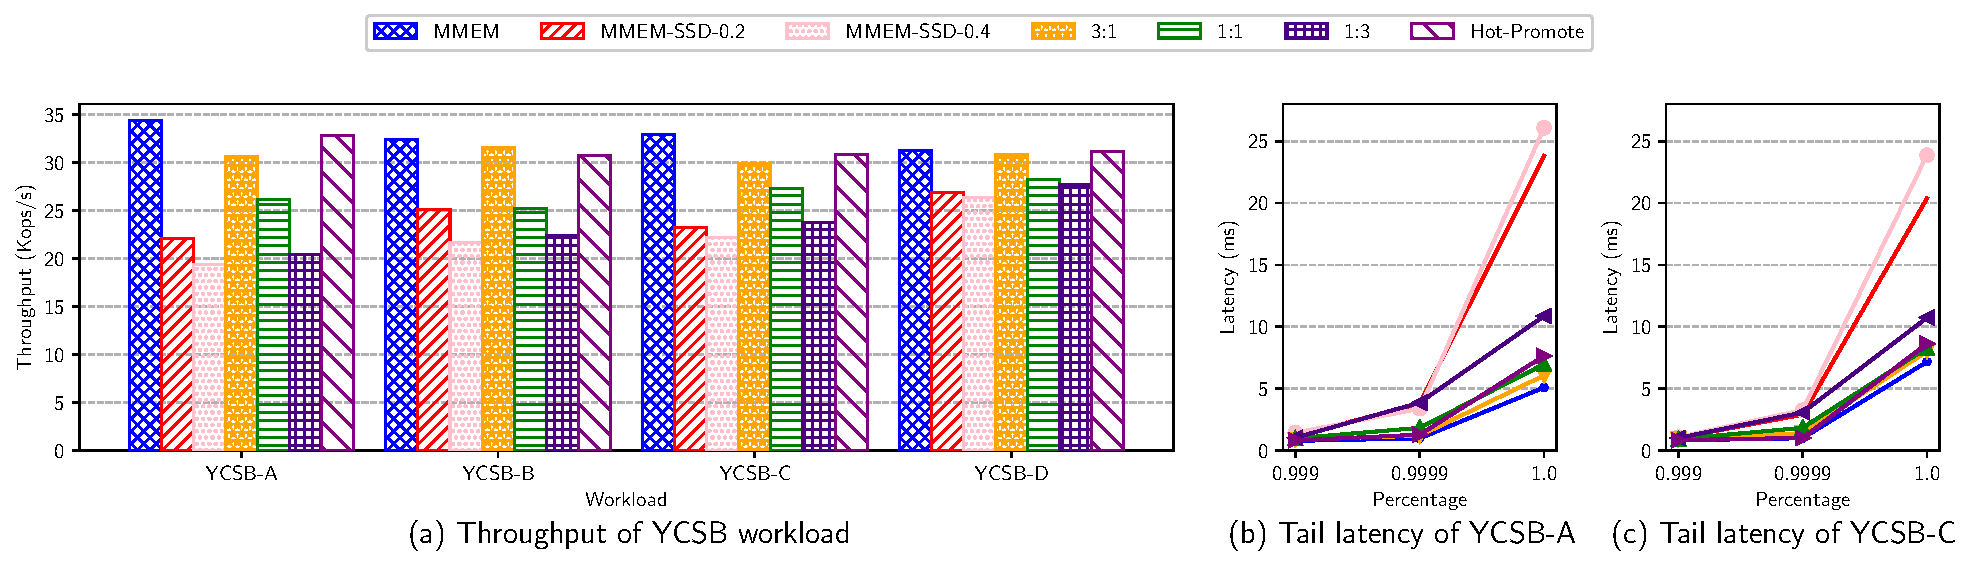
\includegraphics[width=1\textwidth]{fig/cxl/redis_ycsb_cxl.pdf}
  \caption[KeyDB YCSB latency and throughput under different configurations]{\textbf{KeyDB YCSB latency and throughput under different configurations.} (a) Average throughput of four YCSB workload under different system configuration. (b) Tail latency of YCSB-A (c) Tail latency CDF of YCSB-C, both reported by the YCSB client~\cite{YCSB}.}
  \label{fig:ycsb_cxl}
\end{figure*}

One of the most significant advantages of integrating CXL memory into modern computing systems is the potential for significantly larger memory capacities. To highlight the benefits, we focus on three specific use cases: (1) in-memory key-value stores, a commonly used application in data centers, (2) big data analytics applications, and (3) elastic computing from cloud providers.

\subsection{In-memory Key-Value Stores}
\label{ssec:keydb}
Redis~\cite{redis} is a widely-used open-source in-memory key-value store and one of the most popular NoSQL databases. Redis employs a user-defined parameter, \texttt{maxmemory}, to limit memory allocation for storing user data. Similar to traditional memory allocators (e.g., malloc()), Redis may not release memory back to the system after key deletion, particularly when deleted keys reside on memory pages with active ones. As a result, memory provisioning must account for peak demand, making memory capacity a significant bottleneck for Redis deployments in data centers~\cite{manageredis}. Google Cloud recommends keeping memory usage below $80\%$~\cite{googlecloud}, while other sources suggest a $75\%$ limit~\cite{manageredis}.

Due to the substantial infrastructure costs associated with memory-only deployment, Redis Enterprise~\cite{redisenterprise}, a commercial variant supported by leading cloud platforms (e.g., AWS, Google Cloud, Azure), introduces "Auto Tiering"~\cite{redisautotiering}, allowing data overflow to SSDs. This provides an economically viable solution for expanding database capacity beyond RAM limits. Given that Redis Enterprise is not available on our experimental platform, we use KeyDB as an alternative. KeyDB extends Redis's capabilities by integrating KeyDB Flash, which uses RocksDB for persistent storage. The FLASH feature ensures all data is written to disk for persistence, while hot data remains in both memory and disk.

\subsubsection{Methodology and Software Configurations}

In this study, we explore the performance impact of maximizing memory utilization on a KeyDB server. We deploy a single KeyDB instance on a CXL-enabled server configured with seven \textit{server-threads}. Unlike Redis's single-threaded model, KeyDB improves performance by allowing multiple threads to run the standard Redis event loop, effectively simulating several Redis instances in parallel. To minimize potential OS overhead, we disable Sub-NUMA Clustering (SNC) and Transparent Hugepages, and we enable memory overcommitting within the kernel. For KeyDB FLASH, all forms of compression in RocksDB are disabled to reduce software overhead. 

Our empirical evaluation utilizes the YCSB benchmark, testing four distinct workloads:
\begin{enumerate}[leftmargin=*, itemsep=0pt]
    \item \textbf{YCSB-A} ($50\%$ read, $50\%$ update) for update-intensive scenarios,
    \item \textbf{YCSB-B} ($95\%$ read, $5\%$ update) for read-heavy operations,
    \item \textbf{YCSB-C} ($100\%$ read) for read-only tasks,
    \item \textbf{YCSB-D} ($95\%$ read, $5\%$ insert) to simulate workloads accessing the most recent data.
\end{enumerate}
These workloads are evaluated under different system configurations as detailed in Table~\ref{tab:swconfig}. For consistency, we use "MMEM" to refer to main memory, distinguishing it from CXL memory. For configurations involving SSD spillover, we adjust the \texttt{maxmemory} parameter to match the portion of the workload expected to remain in memory. For Hot-Promote, we use \texttt{numactl} to distribute half of the dataset across CXL memory while limiting the main memory usage to half of the dataset size. The experiments utilize a key-value size of $1$ KB, the YCSB default, with a Zipfian distribution for workloads A-C and the latest distribution for workload D. The total working set size is $512$ GB.


\begin{table}[!t]
  \centering
  %\bgroup
  \small
  %\def\arraystretch{0.95}%
  \begin{tabular}{|p{0.22\linewidth} | p{0.65\linewidth}|} 
        \hline
        Configuration & Description \\\hline
        \texttt{MMEM} & Entire working set in main memory. \\\hline
        \texttt{MMEM-SSD-0.2} & $20\%$ of the working set is spilled to SSD. \\\hline
        \texttt{MMEM-SSD-0.4} & $40\%$ of the working set is spilled to SSD. \\\hline
        \texttt{3:1} & Entire working set in memory ($75\%$ MMEM + $25\%$ CXL, 3:1 interleaved). \\\hline
        \texttt{1:1} & Entire working set in memory ($50\%$ MMEM + $50\%$ CXL, 1:1 interleaved). \\\hline
        \texttt{1:3} & Entire working set in memory ($25\%$ MMEM + $75\%$ CXL, 1:3 interleaved). \\\hline
        \texttt{Hot-Promote} & Entire working set in memory ($50\%$ MMEM + $50\%$ CXL), with hot page promotion kernel patches discussed in \S\ref{sec:background}. \\\hline
  \end{tabular}
  %\egroup
  \caption[Configurations used in capacity experiments]{\textbf{Configurations used in capacity experiments.} }
  \label{tab:swconfig}
\end{table}

\subsubsection{Analysis}
Figure~\ref{fig:ycsb_cxl} provides insights into the throughput variations across different configurations. Notably, regardless of the specific workload, running the entire workload on MMEM consistently delivers the highest throughput. This result can be attributed to our workload being primarily constrained by memory capacity rather than memory bandwidth. The Hot-Promote configuration, which utilizes the Zipfian distribution to identify frequently accessed keys (hot pages) and migrate them from CXL to MMEM, performs nearly as well as running the workload entirely on MMEM. This highlights the effectiveness of the Hot-Promote approach in optimizing performance.

In contrast, interleaving data access between CXL and MMEM results in a noticeable performance decrease, with a slowdown of $1.2$x to $1.5$x compared to running the workload entirely on MMEM. This performance drop is primarily due to the higher access latency associated with CXL, as demonstrated in the tail latency plots for workload A and workload C (Figure~\ref{fig:ycsb_cxl}). The MMEM-SSD-0.2 and MMEM-SSD-0.4 configurations exhibit the poorest performance, showing a slowdown of approximately $1.8$x compared to the pure MMEM solution and $1.55$x compared to the CXL interleaving solution. This degraded performance is mainly due to the high access latency required to retrieve data from the SSD.

It is important to note that our choice of a Zipfian distribution ensures that the working set is largely cached in MMEM. If the keys were distributed uniformly, we would expect even worse performance due to the increased frequency of SSD accesses.

\subsubsection{Insights}
Our study demonstrates that the additional memory capacity provided by CXL can be a game-changer for applications like key-value stores, which are traditionally constrained by MMEM’s limited capacity. Moreover, intelligent scheduling policies such as Hot-Promote further enhance the benefits by optimizing performance across multiple memory types while also reducing operational costs.

\subsection{Spark SQL}
\begin{figure}[t]
\centering
 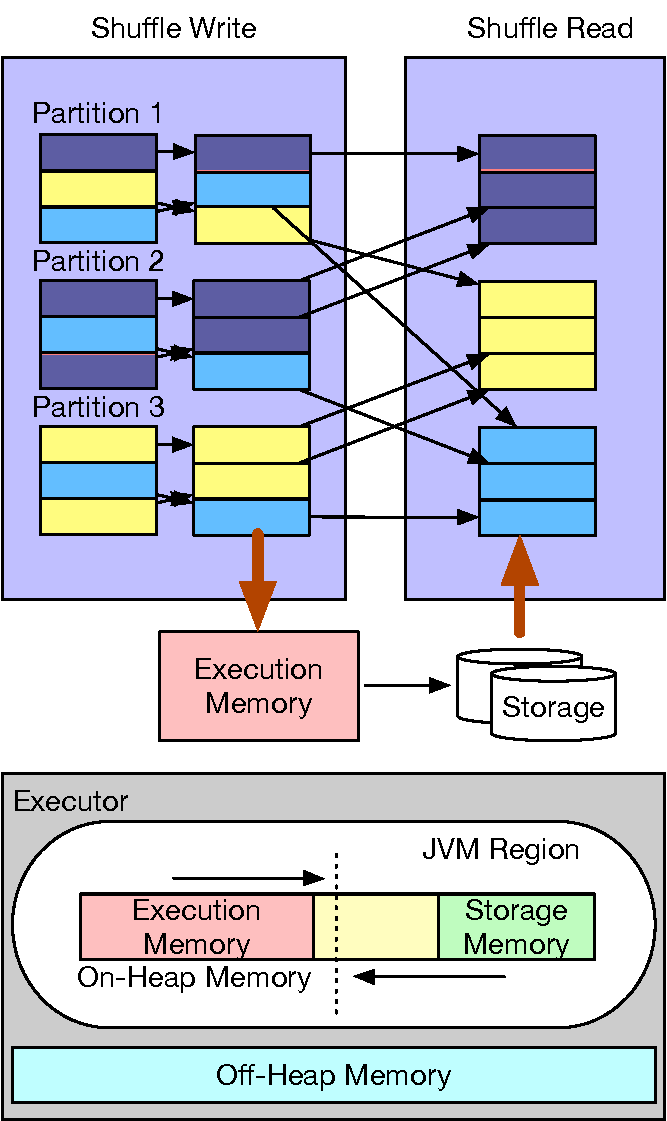
\includegraphics[width=0.3\columnwidth]{fig/cxl/spark.pdf}
  \caption[Spark memory layout and shuffle spill]{\textbf{Spark memory layout and shuffle spill.} Each Spark executor possesses a fixed-size On-Heap memory, which is dynamically divided between execution and storage memory. If there is insufficient memory during shuffle operations, the Spark executor will spill the data to the disk.}
\label{fig:eval_spark_0}
\end{figure}
Big Data plays a crucial role in workloads managed by data centers. Due to the vast scale of data involved in Big Data analytical applications, memory capacity often becomes a bottleneck to performance~\cite{sparkmemory}. Consider Spark~\cite{spark}, one of the most widely used Big Data platforms: A typical query requires shuffling data from multiple tables to process the next stage. Operations like \textit{reduceByKey()} first partition data by key, then execute reduce operations on each key. This shuffling process involves significant disk I/O and network communication between nodes, introducing considerable overhead to the query. In some cases, the performance of shuffling can dominate the overall workload performance~\cite{PSACS}.

During the shuffling process (Fig.~\ref{fig:eval_spark_0}), memory usage can exceed the available capacity or certain thresholds (e.g., \texttt{spark.shuffle.memoryFraction}). When this occurs, Spark can be configured to spill data to disk to avoid out-of-memory failures. However, since disk I/O is orders of magnitude slower than memory, this can significantly degrade the workload’s performance.


\begin{figure*}[t]
\centering
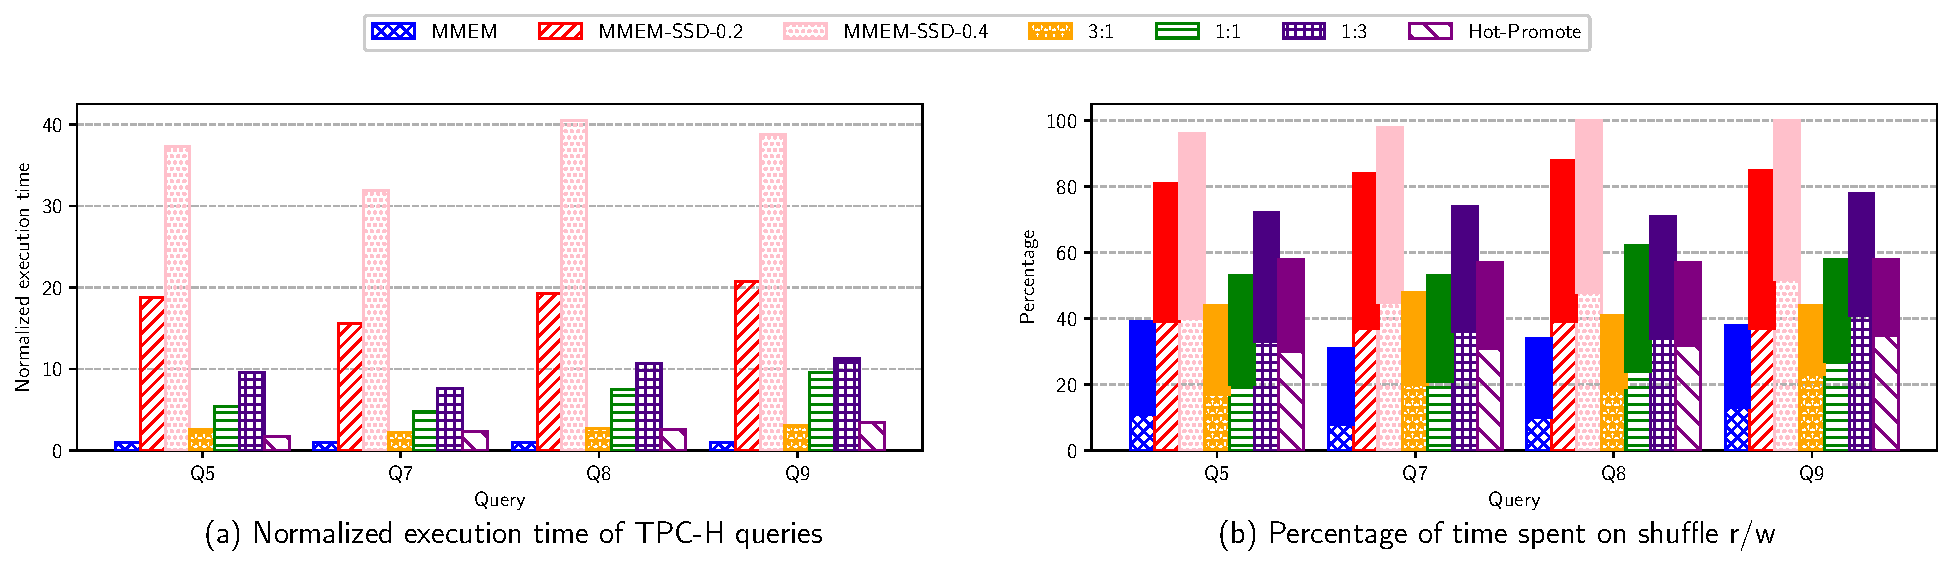
\includegraphics[width=1\textwidth]{fig/cxl/spark_cxl.pdf}
  \caption[Spark execution time and shuffle percentage]{\textbf{Spark execution time and shuffle percentage.} (a) Execution time of each TPC-H query normalized to the execution time running on MMEM. (b) The percentage of time spent of shuffle operation for each query. The solid bars represent shuffle writes, while hollow bars represent shuffle reads.}
\label{fig:eval_spark_1}
\end{figure*}

\subsubsection{Methodology and Software Configurations}

In this experiment, we aim to evaluate whether we can reduce the number of servers required for a specific workload with minimal impact on overall performance. Thus, we compare the performance of Spark running TPC-H~\cite{tpch} on three servers without CXL memory expansion against two servers equipped with CXL memory expansion. We assume that the maximum amount of MMEM per server is $512$ GB, so with three servers, we have a total of $1.5$ TB of MMEM and $1$ TB of CXL memory.

To trigger data spill within the workload, we configure Spark with 150 executors. Each Spark executor is allocated $1$ core and $8$ GB of memory, resulting in a total memory usage of $1.2$ TB and 150 cores. We generate a $7$ TB TPC-H dataset. The configuration settings detailed in Table~\ref{tab:swconfig} are applied as follows:

\begin{itemize}
  \item \textbf{MMEM only}: We allocate $50$ Spark executors and $400$ GB of memory on each of the \textbf{three} servers. In this scenario, no data is spilled to disk, as each executor has sufficient memory.
  
  \item \textbf{MMEM/CXL interleaving}: We distribute the same number of executors ($150$) across the \textbf{two} CXL-enabled servers, which have $1$ TB of CXL memory ($512$ GB from each of two CXL cards) and $1$ TB of MMEM ($512$ GB each). For instance, in a configuration where MMEM and CXL memory usage is balanced (1:1 ratio), we allocate $75$ executors to $600$ GB of MMEM and $75$ executors to $600$ GB of CXL memory. In this case, data spill to disk is negligible.
  
  \item \textbf{Spill to SSD}: To simulate conditions where Spark executors run out of memory and need to spill data to SSD storage, we restrict memory allocation to either $80\%$ or $60\%$ of the total $1.2$ TB MMEM, leading to approximately $320$ GB and $500$ GB of data being spilled to disk, respectively.
  
  \item \textbf{Hot-Promote}: Similar to the KeyDB experiment (\S\ref{ssec:keydb}), this configuration migrates hot data from CXL to MMEM.
\end{itemize}

We selected four TPC-H queries ($Q5$, $Q7$, $Q8$, and $Q9$), which are known for their intensive data shuffling demands~\cite{PSACS}, to evaluate our setup. Our measurements focus solely on the execution time of these queries, excluding data preparation and server setup times. SNC was disabled on all servers.

\subsubsection{Analysis}

Figure~\ref{fig:eval_spark_1}(a) illustrates variations in total execution time across different configurations. To provide a clear comparison, we normalized the total execution time against the best-case scenario, which is running the entire workload in MMEM. Similar to the KeyDB experiments, the interleaving approach results in a performance slowdown ranging from $1.4$x to $9.8$x compared to the optimal MMEM-only scenario, though it uses fewer servers. This performance degradation worsens as a larger proportion of memory is allocated to CXL. Nevertheless, it is crucial to note that even with this slowdown, the interleaving approach is significantly faster than spilling data to SSDs. Figure~\ref{fig:eval_spark_1}(b) shows that data shuffling exacerbates the total execution time due to intensified data spill issues.

A notable difference between the KeyDB and Spark experiments is the performance of the Hot-Promote configuration. While it performs well in KeyDB, the Spark SQL experiment reveals a more than $34\%$ slowdown compared to MMEM. Unlike the Zipfian distribution, which efficiently promotes hot keys from CXL to DDR, Spark SQL encounters considerable thrashing behavior within the kernel. Upon investigation, we traced the root cause to the hot page selection patch~\cite{hot}. In its initial version, a sysctl parameter (\texttt{kernel.numa\_balancing\_promote\_rate\_limit\_MBps}) was used to control the maximum promotion/demotion throughput. Later versions introduced an automatic threshold adjustment feature to balance the speed of promotion with migration costs. However, this automatic adjustment mechanism seems inadequate for the Spark SQL workload, which demonstrates reduced data locality and challenges the kernel's ability to efficiently promote frequently accessed pages. This issue is consistent with prior findings~\cite{demystify}.

\subsubsection{Insights}

Our research indicates that utilizing CXL memory expansion offers a cost-effective solution for data center applications. A detailed theoretical examination of the Abstract Cost Model is postponed to \S\ref{sec:cost}. While the hot-promote patch shows significant advantages in key-value store workloads, its performance is notably lacking in Spark experiments. As system developers work to enhance software support for CXL within the kernel, they should proceed with caution. System-wide policies can have varied impacts depending on the specific characteristics of different applications.

\subsection{Spare Cores for Virtual Machine}

\begin{table*}[!]
  \centering
  %\bgroup
  \small
  %\def\arraystretch{0.95}%
  \begin{tabular}{c|c|c|c|c} 
        \hline
        Year & CPU & Max vCPU  &  Max memory & Required Memory \\
        & & per server &  \textbackslash TB & ($1:4$) \textbackslash TB\\\hline
        $2021$ & IceLake-SP\cite{icelakecores} & $160$  & $4$ & $0.64$ \\\hline
        $2022$ (delayed) & Sapphire Rapids\cite{sprcores} & $192$  & 	$4$ & $0.768$ \\\hline
        $2023$ (delayed) & Emerald Rapids\cite{emeraldrapidscores} & $256$ & $4$ & $1$ \\\hline
        $2024$+  & Sierra Forest\cite{sierraforestcores} & $1152$ & $4$ & $4.5$ \\\hline
        $2025$+ & Clearwater Forest\cite{clearwatercores} & $1152$ & $4$ & $4.5$ \\\hline
  \end{tabular}
  %\egroup
  \caption[Intel Processor Series]{\textbf{Intel Processor Series.} }
  \label{tab:amd}
\end{table*}

One widely-used application within Infrastructure-as-a-Service (IaaS) is Elastic Computing~\cite{elasticcomputing}, where cloud service providers (CSPs) offer computational resources to users through virtual machines (VMs) or container instances. Given the diverse requirements of users, CSPs typically offer various instance types, each configured with different CPU cores, memory, disk, and network capacities. A commonly employed "optimal" CPU-to-memory ratio is $1:4$, as recommended by AWS~\cite{awsm7a, awsm7i}. For instance, an instance with $128$ vCPUs would generally have $512$ GB of DDR memory.

Advancements in server processor architecture and chiplet technology have rapidly increased the number of cores available in a single processor package, driven largely by CSPs' desire to lower per-core costs. Consequently, vCPU counts in 2-socket servers have increased from $160$ to $256$ over the past two years (Table~\ref{tab:amd}), with projections reaching as high as $1152$ vCPUs per server by 2025.

This surge in vCPUs exacerbates memory capacity bottlenecks, which are limited by DDR slot availability, DRAM density, and the cost of high-density DIMMs. For example, Intel's Sierra Forest Xeon supports up to $1152$ vCPUs but is constrained by motherboard design to less than $4$ TB of memory—falling short of the typical $4.5$ TB required for VM provisioning~\cite{1dpc}. This shortfall complicates the maintenance of a cost-effective vCPU-to-memory ratio, leading to underutilized vCPUs and revenue losses for CSPs. CXL memory expansion offers a solution by enabling memory capacity to scale beyond DDR limitations, thereby optimizing vCPU utilization and mitigating revenue losses for CSPs.

\subsubsection{Methodology and Software Configurations}

To evaluate the performance impact when an application runs entirely on CXL memory, we replicate the KeyDB configuration from earlier experiments (\S\ref{ssec:keydb}). Using \textit{numactl}, we allocate the KeyDB instance exclusively to either MMEM or CXL memory. The workload for this evaluation is YCSB-C, which features $1$ KB key-value pairs and a total dataset size of $100$ GB. SNC is disabled in all configurations.

\subsubsection{Analysis}

The Cumulative Distribution Function (CDF) of read latency (Fig.~\ref{fig:eval_vm_0}) shows that applications running on CXL memory experience a latency penalty of $9\%-27\%$, which is less than the raw data fetching latency observed in \S\ref{sec:micro}. This difference is due to processing latency within Redis. Furthermore, the throughput of running the entire workload on CXL memory is approximately $12.5\%$ lower than that of MMEM, as shown in Fig.~\ref{fig:eval_vm_1}.

Consider a server operating at a suboptimal vCPU-to-memory ratio of $1:3$:
\begin{enumerate}[leftmargin=*, itemsep=0pt]
    \item Due to insufficient memory, only $75\%$ of the available vCPUs can be sold at the optimal $1:4$ ratio, resulting in a $25\%$ revenue loss. By implementing CXL memory expansion, CSPs can sell the remaining $25\%$ of vCPUs at the optimal ratio.
    \item Our benchmarks show that instances running on CXL memory perform $12.5\%$ slower than those running on DDR memory for common workloads like Redis. Assuming a $20\%$ price discount on such instances, CSPs can still recover approximately $80\%$ of the lost revenue, resulting in a ~$27\%$ improvement in total revenue ($20/75 = 26.77\%$).
\end{enumerate}


\begin{figure}[t]
  \center
  \subfigure[CDF of KeyDB YCSB-C]{
    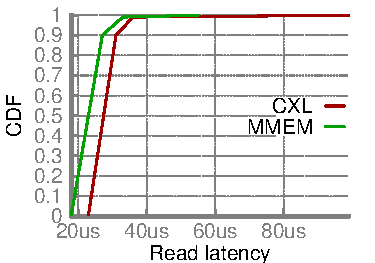
\includegraphics[width=0.4\textwidth]{fig/cxl/new_read_latency_cdf.pdf}
    \label{fig:eval_vm_0}}
  \subfigure[Throughput of KeyDB YCSB-C]{
    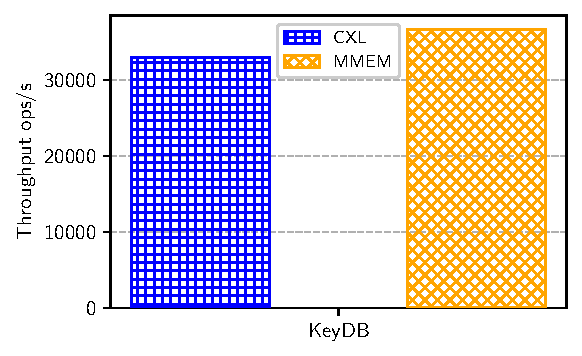
\includegraphics[width=0.4\textwidth]{fig/cxl/redis_ycsb.pdf}
    \label{fig:eval_vm_1}}
\caption[KeyDB Performance with YCSB-C on CXL/MMEM]{\textbf{KeyDB Performance with YCSB-C on CXL/MMEM.}}
\end{figure}


\subsubsection{Insights}
Given the vast scale of Elastic Computing Service (ECS) applications in public clouds, the potential benefits of CXL memory expansion are considerable. However, maintaining an optimal virtual CPU (vCPU) to memory ratio, traditionally set at $1:4$, becomes increasingly complex with the rapid growth in processor cores. Although this ratio is a standard, its applicability in future cloud computing paradigms is being reevaluated. For example, Bytedance's Volcano Engine Cloud~\cite{volcano} demonstrates variability in resource allocation by offering different ratios: $1:4$ for general-purpose workloads, $1:2$ for compute-intensive tasks, and $1:8$ for memory and storage-intensive applications. The introduction of CXL memory expansion and pooling into these established ratios presents an intriguing area of exploration, raising important questions about the adaptability of cloud providers to evolving hardware capabilities and the subsequent effect on resource allocation standards.

\section{Memory Bandwidth-Bound Applications}
\label{sec:bandwidth}

Another advantage of CXL memory expansion is its potential to provide additional memory bandwidth. We use Large Language Model (LLM) inference as an example to demonstrate how this can benefit real-world applications.

Recent research on LLMs~\cite{gpt4} highlights that LLM inference is both memory-capacity and memory-bandwidth intensive. The limited capacity of GPU memory constrains the batch size of LLM inference jobs and reduces computational efficiency, as LLM models are highly memory-demanding. On the other hand, while CPU memory offers larger capacity, it suffers from lower bandwidth compared to GPU memory. The extra bandwidth and capacity offered by CXL memory make it a promising solution for alleviating these bottlenecks.

For instance, a CPU-based LLM inference job could benefit from the additional bandwidth provided by CXL memory. Similarly, a CXL-enabled GPU device could leverage the extra memory capacity from a disaggregated memory pool. Due to the current lack of CXL support in GPU devices, we focus on CPU-based LLM inference in our experiments to assess the potential impact of CXL memory’s extra bandwidth. Moreover, since LLM inference applications are generally agnostic to the underlying memory technologies, our findings and implications should also apply to future CXL 2.0/3.0 devices.


\begin{figure}[t]
\centering
 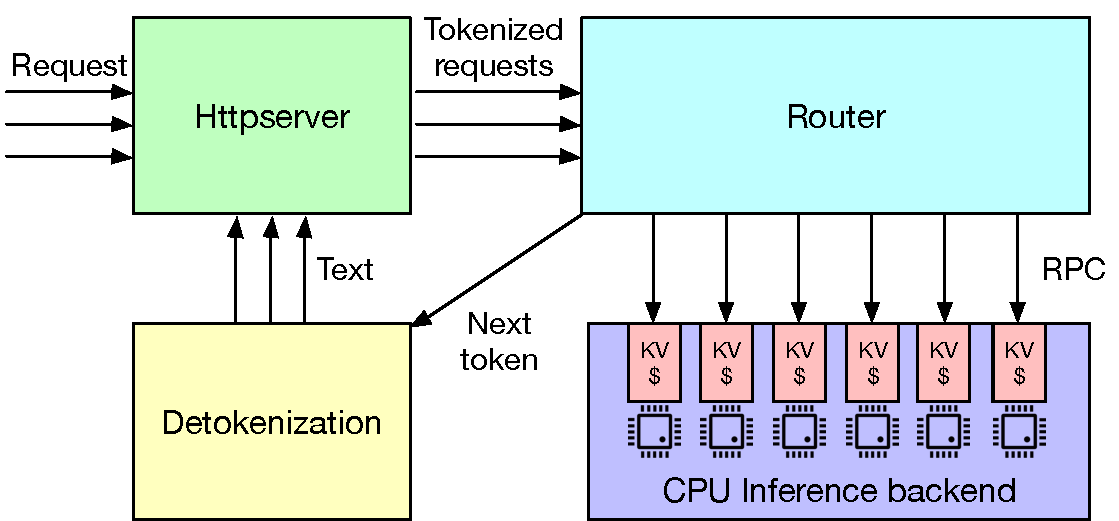
\includegraphics[width=0.6\columnwidth]{fig/cxl/llm.pdf}
  \caption[LLM inference framework]{\textbf{LLM inference framework.} The Httpserver receive requests and forward the tokenized requests to the CPU inference backend. The CPU inference backend serves the requests and reply the next token.}
\label{fig:llm-framework}
\end{figure}

\begin{figure*}[h!]
\centering
\subfigure[LLM inference serving rate vs. number of threads]{
  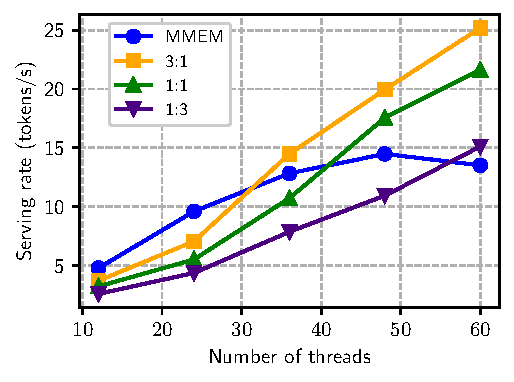
\includegraphics[width=0.31\textwidth]{fig/cxl/llm_serving.pdf}
  \label{fig:eval-llm-1}
}
\subfigure[Memory bandwidth vs. number of threads for a single backend]{
  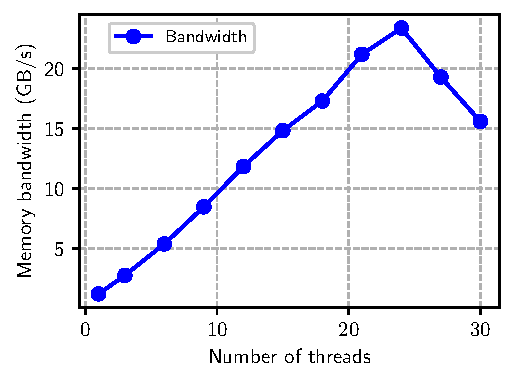
\includegraphics[width=0.31\textwidth]{fig/cxl/llm_bandwidth.pdf}
  \label{fig:eval-llm-2}
}
\subfigure[Memory bandwidth vs. KVcache size for a single backend]{
  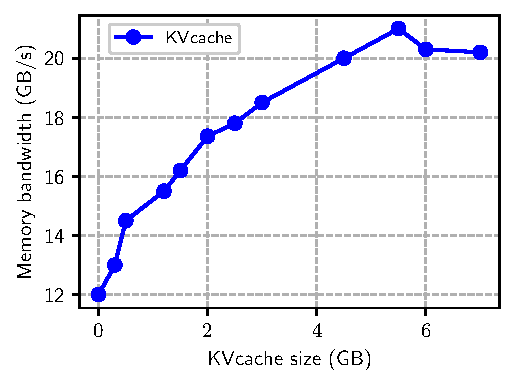
\includegraphics[width=0.31\textwidth]{fig/cxl/kvcache.pdf}
  \label{fig:eval-llm-3}
}
\caption[CPU LLM inference]{\textbf{CPU LLM inference.} }
\end{figure*}
\paragraphb{LLM Inference Framework}
Mainstream Large Language Model (LLM) inference frameworks, such as vLLM~\cite{vllm} and LightLLM~\cite{lightllm}, do not natively support CPU-based inference. Recently, Intel introduced the Q8chat LLM model~\cite{q8chat}, trained using their 4th Generation Intel Xeon® Scalable Processors. However, the inference code for Q8chat is not yet publicly available. 

To address this gap, we developed an inference framework based on the open-source LightLLM framework~\cite{lightllm}, replacing its backend with a CPU inference backend. Figure~\ref{fig:llm-framework} illustrates our implementation. In our framework, an HTTP server frontend receives LLM inference requests and forwards the tokenized requests to a router. The router distributes these requests to different CPU backend instances, each equipped with a Key-Value (KV) cache~\cite{kvcache}, a widely-used technique in LLM inference.

It is important to note that KV caching, despite its name, differs from traditional key-value stores in system architecture. KV caching occurs during multiple token generation steps within the decoder. During decoding, the model begins with a sequence of tokens, predicts the next token, appends it to the input, and repeats the process. This is how models like GPT~\cite{gpt4} generate responses. The KV cache stores key and value projections used as intermediate data during decoding to avoid recomputation for each token generation. Prior research~\cite{kvcache} has shown that KV caching is typically memory-bandwidth bound, as each sequence in the batch has its own unique KV cache, and different requests do not share this cache due to sequences being stored in separate contiguous memory spaces~\cite{vllmpaper}.

\subsection{Methodology and Software Configurations}
To investigate the benefits of CXL memory extension for applications with high memory bandwidth demands and limited MMEM bandwidth, we use an SNC-4 configuration to partition a single CPU into four sub-NUMA nodes. Each sub-NUMA node is equipped with two DDR5-4800 memory channels, which results in early memory bandwidth saturation at $67$ GB/s (\S\ref{sec:micro}). We evaluate three different interleaving policies ($3$:$1$, $1$:$1$, $1$:$3$), as detailed in Table~\ref{tab:swconfig}. The CPU inference backend is configured with 12 CPU threads, with memory allocation strictly bound to a single sub-NUMA domain. Each domain includes two DDR5-4800 channels and a $256$ GB A1000 CXL memory expansion module via PCIe. By binding allocations to a single node, we ensure the early saturation of DDR5 channels. 

For our experiments, we use the Alpaca 7B model~\cite{alpaca}, an extension of the LLaMA 7B model, which requires 4.1 GB of memory. The workload, derived from the LightLLM framework~\cite{lightllm}, includes a variety of chat-oriented questions. A single-threaded client machine on a baseline server sends HTTP requests with different LLM queries to simulate real-world conditions. The client ensures continuous operation of the CPU inference backends by maintaining a constant stream of requests. The prompt context is set to 2048 bytes to ensure a minimum inference response size. We progressively increase the number of CPU inference backends to monitor the LLM inference serving rate (measured in tokens/s).

\subsection{Analysis}
Figure~\ref{fig:eval-llm-1} shows the inference serving rates across different memory configurations as the number of CPU inference backends increases. Initially, the serving rate improves almost linearly with available memory bandwidth. However, at 48 threads, MMEM bandwidth saturation limits the serving rate, while the interleaving configurations benefit from additional CXL bandwidth for continued scaling. With a high number of inference threads (60), a MMEM:CXL = $3$:$1$ interleaving configuration outperforms the MMEM-only setup by $95\%$.

Among the interleaving policies, configurations with a higher proportion of data in main memory demonstrate better inference performance. Interestingly, we observe that beyond 64 threads, operating entirely on main memory is $14\%$ less effective than a MMEM:CXL ratio of $1$:$3$. This result is surprising given CXL’s higher latency and lower memory bandwidth (\S~\ref{sec:micro}). Figure~\ref{fig:eval-llm-2} shows the memory bandwidth utilization, as measured by the Intel Performance Counter Monitor (PCM)~\cite{pcm}, with increasing CPU thread counts. Bandwidth utilization grows linearly with thread count, plateauing at $24.2$ GB/s for 24 threads. This trend allows us to estimate a bandwidth of approximately $63$ GB/s at 60 threads, reaching $82\%$ of the theoretical maximum. Our microbenchmark results (\S\ref{sec:micro}) suggest that this level of bandwidth utilization could cause significant latency spikes, corroborating the hypothesis that bandwidth contention plays a critical role in performance degradation.

Bandwidth contention may arise from loading the LLM model or accessing the KV cache. By adjusting the prompt context to infinity, the LLM model continuously generates new tokens for storage in the KV cache. Figure~\ref{fig:eval-llm-3} illustrates the relationship between KV cache size and memory bandwidth consumption. The initial memory bandwidth of approximately $12$ GB/s originates from I/O threads loading the model from memory. As the KV cache stores more tokens, memory usage increases linearly. However, bandwidth utilization plateaus around $21$ GB/s.

\subsection{Insights}
Current tiered memory management in the kernel does not account for memory bandwidth contention. For a workload that utilizes a high percentage of MMEM bandwidth (e.g., $70\%$), existing page migration policies (\S\ref{sec:background}) tend to move data from slower tiered memory (e.g., CXL) into MMEM, assuming sufficient memory capacity is available. As more data is written to MMEM, memory bandwidth utilization may rise to $90\%$, exponentially increasing access latency and causing a slowdown in the workload. This scenario is likely to occur in memory-bandwidth-bound applications, such as LLM inference. Therefore, the definition and management of tiered memory need to be reconsidered to address bandwidth contention effectively.






\section{Cost Implications}
\label{sec:cost}
\begin{table}[btp!]
  \centering
  \footnotesize
  \begin{tabular}{l|l}
    \hline
    Parameter & Description \\ \hline
    $P_s$  & \makecell[l]{Throughput when (almost) entire working set is spilled to SSD on a server. \\ Normalized to 1 in the cost model.}  \\  \hline
    $R_d$ & \makecell[l]{Relative throughput when the entire working set is in main memory on a server, normalized to $P_s$.}   \\ \hline
    $R_c$ & \makecell[l]{Relative throughput when the entire working set is in CXL memory on a server, normalized to $P_s$.}  \\ \hline
    $D$ & \makecell[l]{The MMEM capacity allocated to each server. For completeness only, not used in cost model.} \\ \hline
    $C$ & \makecell[l]{The ratio of main memory to CXL capacity on a CXL server. \\ E.g. 2 means the server has 2x MMEM capacity than CXL memory.} \\ \hline
    $N_{baseline}$ & Number of servers in the baseline cluster. \\ \hline
    $N_{cxl}$ & \makecell[l]{Number of servers in the cluster with CXL memory to deliver the same performance as the baseline.} \\ \hline
    $R_t$ & \makecell[l]{Relative TCO comparing a server equipped with CXL memory vs. baseline server. \\ E.g. If a server with CXL memory costs $10\%$ more than the baseline server, this parameter is $1.1$.} \\ \hline 
  \end{tabular}
  \caption[Parameters of our Abstract Cost Model]{\textbf{Parameters of our Abstract Cost Model.}}
  \label{tab:roi}
\end{table}

Our comprehensive analysis in previous sections (\S\ref{sec:capacity}, \S\ref{sec:bandwidth}) demonstrates that the adoption of CXL memory expansion offers substantial benefits for data center applications, including comparable performance alongside significant operational cost savings. However, a major challenge in adopting innovative technologies like CXL lies in determining its Return on Investment (ROI). While detailed technical specifications and benchmark performance results are often available, accurately forecasting the Total Cost of Ownership (TCO) savings remains difficult. This is compounded by the complexity of running production-scale benchmarks and the limited availability of CXL hardware. Traditional cost models~\cite{CXLPoolCost}, which aim to provide such forecasts, typically require extensive internal data that is often sensitive and inaccessible. To address this challenge, we propose an Abstract Cost Model that estimates TCO savings without relying on internal or sensitive information. This model leverages a small set of metrics obtainable through microbenchmarks, along with empirical values that are easier to approximate or access, providing a viable approach to evaluating the economic feasibility of CXL technology adoption.

To illustrate the application of our Abstract Cost Model, we use a capacity-bound application (Spark SQL) as an example. However, this methodology can be extended to other types of workloads. For Spark SQL applications, the additional memory capacity provided by CXL reduces the amount of data spilled to SSD, resulting in improved throughput and performance. This, in turn, means that fewer servers are required to meet the same performance target.

Given that the workload maintains a relatively consistent memory footprint (i.e., the size of the active dataset) during execution, we can approximate the execution time of the workload by dividing it into three distinct segments:
\begin{enumerate}[leftmargin=*, itemsep=0pt]
  \item The segment processed with data stored in MMEM,
  \item The segment processed with data stored in CXL memory,
  \item The segment processed with data offloaded to SSD storage.
\end{enumerate}

We begin by collecting the following measurements from microbenchmarks on a single server:
\begin{itemize}[leftmargin=*, itemsep=0pt]
  \item \textbf{Baseline performance ($P_s$)}: Measure the throughput when (almost) the entire working set is spilled to SSD. While the absolute number is not directly used in our cost model, we normalize this value to 1 for comparison.
  \item \textbf{Relative performance with the entire working set in MMEM ($R_d$)}: Using the same workload, measure the throughput when the entire working set resides in MMEM. Normalize this value to $P_s$ to express the relative performance improvement (i.e., how much faster compared to the baseline).
  \item \textbf{Relative performance with the entire working set in CXL memory ($R_c$)}: Using the same workload, measure the throughput when the entire working set resides in CXL memory. Normalize this value to $P_s$ to express the relative performance compared to the baseline.
\end{itemize}

We then formulate our cost model using the parameters summarized in Table~\ref{tab:roi}. For a working set size of $W$, the execution time of the baseline cluster can be approximated as the sum of two segments: (1) the segment executed with data in MMEM and (2) the segment executed with data spilled to SSD.



$$
T_{baseline} = \frac{N_{baseline} D}{R_d} + (W - N_{baseline}D)
$$

The execution time of the cluster with CXL memory could be approximated in a similar way.
It includes the segment that is executed with data in main memory, in CXL memory, and spilled to SSD respectively.

$$ T_{cxl} = \frac{N_{cxl} D}{R_d} + \frac{N_{cxl} D}{CR_c} + (W - N_{cxl} D - \frac{N_{cxl} D}{C}) $$

To meet the same performance target, $T_{baseline} = T_{cxl}$:

% Under the same SLA conditions, $ T1 = T2 $, thus:

$$
\frac{N_{baseline} D}{R_d} - N_{baseline} D = \frac{N_{cxl} D}{R_d} + \frac{N_{cxl} D}{CR_c} - N_{cxl} D - \frac{N_{cxl} D }{C}
$$

% After some simple transformations, we have:

% $$ (C+1)/C - (C R_c + R_d) / (C R_c R_d) N_{cxl} = (R_d - 1) / R_d N_{baseline} $$

With some simple transformations, we get the ratio between $N_{cxl}$ and $N_{baseline}$: 
% Comparing the sizes of baseline and CXL clusters, we have:

$$ \frac{N_{cxl}}{N_{baseline}} = \frac{CR_c(R_d - 1)}{R_cR_d(C+1) - C R_c - R_d} $$

TCO saving can then be formulated as follows.

$$
TCO_{saving}=1-\frac{TCO_{cxl}}{TCO_{baseline}}=1-\frac{N_{cxl} R_t}{N_{baseline}}
$$

% \yupeng{TODO: change these numbers}
% Using our Redis experiments(\S\ref{sec:capacity}) as an example, we measure that

For example, suppose $ R_d = 10 $, $R_c = 8 $, $ C = 2 $, we get $\frac{N_{cxl}}{N_{baseline}} = 67.29\%$ from the cost model.
This means that by using CXL memory, we may reduce the number of servers by $32.71\%$.
And if we further assume $R_t=1.1$ (a server with CXL memory costs $10\%$ more than the baseline server), the TCO saving is estimated to be $25.98\%$.

Our Abstract Cost Model provides an easy and accessible way to estimate the benefit from using CXL memory,
providing important guidance to the design of the next-generation infrastructure.

\paragraphb{Extending Cost Model for more realistic scenarios}
In line with previous research \cite{CXLPoolCost}, our Abstract Cost Model is designed to be adaptable, allowing for the inclusion of additional practical infrastructure expenses such as the cost of CXL memory controllers, CXL switches (applicable in CXL 2.0/3.0 versions), PCBs, cables, etc., as fixed constants. However, a notable constraint of our current model is its focus on only one type of application at a time. This becomes a challenge when a data center provider seeks to evaluate cost savings for multiple distinct applications, each with unique characteristics, especially in environments where resources are shared (for instance, through CXL memory pools). This scenario introduces complexity and presents an intriguing challenge, which we acknowledge as an area for future investigation.

\section{Related Work}

As memory-intensive applications like machine learning and High-Performance Computing (HPC) continue to grow, expanding memory capacity and bandwidth has become a critical challenge~\cite{dataintensive, FlatFlash, cxl-ssd}. Compute Express Link (CXL)~\cite{cxl, cxl_azure, cxlcentric} has emerged as a promising solution, offering a novel interconnect technology that connects external memory devices via PCIe, significantly enhancing both memory capacity and bandwidth.

Research on CXL technology is extensive. Studies such as \cite{cxl_azure, cxlcentric, demystify} explore CXL’s potential for resource disaggregation and memory expansion, highlighting its ability to address memory bottlenecks in large-scale applications. However, much of the research relies on simulations~\cite{pond, cxlcentric} or FPGA-based CXL hardware~\cite{demystify, intelfpga, directcxl}, limiting practical insights into production-ready ASIC-based hardware. More recent empirical evaluations, such as \cite{demystify, smt}, have begun to investigate the performance of ASIC-based CXL hardware, offering valuable data on its real-world potential. These studies show that while CXL introduces higher latency compared to local memory, this gap narrows for cross-socket memory access, making CXL a feasible option for memory tiering.

Other work, such as \cite{pond, tpp, directcxl}, has examined the trade-offs between performance and cost in CXL systems, particularly through synthetic benchmarks. For instance, \cite{tpp} investigates kernel-level techniques for promoting hot pages from slower to faster memory tiers to boost performance while maintaining application transparency. Similarly, \cite{CXLPoolCost} introduces cost models for memory pooling in CXL, but further research is needed to evaluate the economic viability of migrating specific workloads to CXL-enabled systems.

\section{Summary}

In this chapter, we provide a comprehensive empirical evaluation of Compute Express Link (CXL) in real-world data center applications, filling a critical knowledge gap left by prior theoretical studies. Our findings reveal both the potential and limitations of CXL, offering actionable recommendations for its ongoing development to better serve data-centric computing environments. Based on our benchmarks, we also develop an Abstract Cost Model that can estimate the TCO savings without relying on internal or sensitive data, providing important guidance to the design of our next generation infrastructure
